
\chapter{Introduction}
	%%Article Purpose

%fundamental

%\chapter{fundamental Theories}
%
%\section{Geometric Optics}
%%optics
Optical fibers are widely used as a medium for telecommuniction and networking because of varity of advantages.It is flexible,especially permits transmission over longer distances and at higher bandwidths (data rates) than other forms of communication. The Fig.\ref{fig:opticfiber} presents a simplest optical fiber and how lights progate in the fiber. 

\begin{figure}[httbp]
\centering
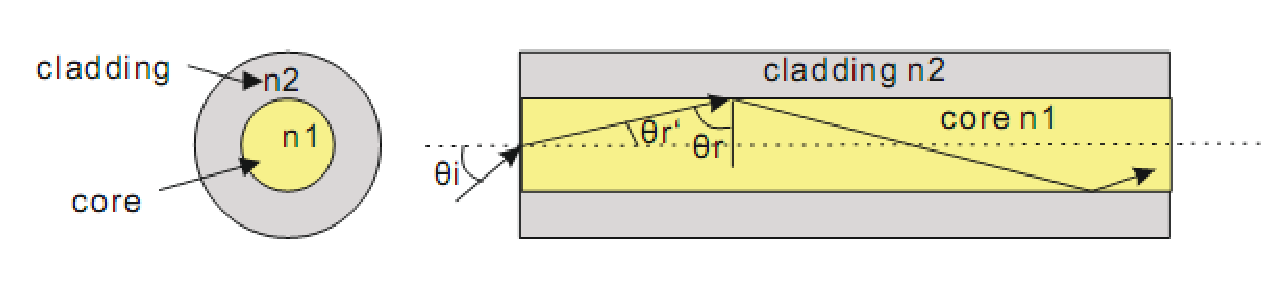
\includegraphics[width=0.8\textwidth]{bilder/opticfiber}
\caption{linght refraction in optic fibers}
\label{fig:opticfiber}
\end{figure}

Optical fiber typically consists of a transparent core with index $n1$ surrounded by a transparent cladding material with a lower index of refraction $n2$. The Light is kept in the core by total internal reflection. This causes the fiber to act as a waveguide.
The principle of the total reflection is explained in \cite{script_FT_TET} with Snell's law. In Fig.\ref{fig:totalreflection} linghts strike a boundary between two different isotropic media with respective refractive indices $n_{1}$ and $n_{2}$ ($n_{1}>n_{2}$), it behaves after Snell's law, which is presented in following mathematical fomular (\ref{eq:snell}).
\begin{figure}[httbp]
\centering
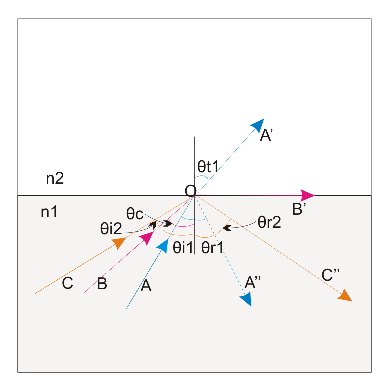
\includegraphics[width=0.6\textwidth]{bilder/totalreflection}
\caption{total reflection}
\label{fig:totalreflection}
\end{figure}

\begin{equation}
n_{1}sin\theta_{i}=n_{2}sin\theta_{t}
\label{eq:snell}
\end{equation}

$\theta_{t}$ is transmission angle or refraction angle.
At a small incidence angle $\theta_{i1}$ a light beam can pass through the boundary and bend to a new course at transmission angle $\theta_{t1}$ in the second meadium.
When the incidence angle is larger than a particular critical angle (\ref{eq:critical_angle}) with respect to the normal to the surface, no light can pass through and all of the light is reflected like (O-C''). In this case the value of $sin\theta_{t}$ in (\ref{eq:sin_transmission_angle}) become larger than one and he mathematical formular of the new transmission angle can be presented by a complex symble $\underline{\theta_{t}}$(\ref{eq:complex_transmission_angle}). $\underline{\theta_{t}}$ is not a real physical angle.

\begin{equation}
\theta_{c}=arcsin(\frac{n_{2}}{n_{1}})
\label{eq:critical_angle}
\end{equation}

\begin{equation}
sin\theta_{t}=\frac{n_{1}}{n_{2}}sin\theta_{i}
\label{eq:sin_transmission_angle}
\end{equation}

\begin{equation}
\underline{\theta_{t}}=\frac{\pi}{2}+j\gamma
\label{eq:complex_transmission_angle}
\end{equation}
with
\begin{equation}
sin\underline{\theta_{t}}=cosh\gamma=\frac{n{1}}{n_{2}}sin\theta_{i},\hspace{2cm}\hfill cos\underline{\theta_{t}}=jsinh\gamma=j\sqrt{cosh^2\gamma-1}
\label{eq:trangle_transmission_angle}
\end{equation}


%Numerical Apertur
Back to the Fig.\ref{fig:opticfiber} the incidence beam originate from the aire into the fiber. There is a maximus coupling angle,so that the beam can be guided under the total reflecting conditions. Its sinus value(\ref{eq:NA}) is called \textbf{Numerical Apertur(NA)}, which indicate the acceptable range of ray beams.

\begin{align}
sin\theta_{i}&=\frac{n_{1}}{n_{0}}sin(90^{o}-\theta_{c})=n_{1}cos\theta_{c} \nonumber\\
&=n_{1}\sqrt{1-sin^{2}\theta_{c}}=n_{1}\sqrt{1-\left(\frac{n_{2}}{n_{1}}\right)^2}=\sqrt{n^2_{1}-n^2_{2}}
\label{eq:NA}
\end{align}

%\newpage
%\section{Gaussian Beam}
%In nature world there is no source of parallel ray. Each beams of lights can be in some ways considered from a simple origin: point light source,which emits light in all directions. Thus a normal light source can not provide a perfect focused beams for optical applications. Laser light (laser radiation)has some very special properties, which very much distinguish it from light with other origins:

\begin{itemize}
\item Laser light is usually delivered in the form of a laser beam, i.e. it propagates dominantly in a well-defined direction with moderate beam divergence. Such a laser beam has a high (sometimes extremely high) degree of spatial coherence. This means that the electric fields at different locations across a beam profile oscillate with a rigid phase relationship. Exactly this coherence is the reason why a laser beam can propagate over long distances without spreading very much in the transverse directions, and why it can be focused to very small spots (high focusability of laser beams).

\item In many but not all cases, laser light also has a high degree of temporal coherence, which is equivalent to a long coherence length. This means that a rigid phase relationship is also maintained over relatively long time intervals, corresponding to large propagation distances (often many kilometers) or to huge numbers of oscillation cycles.
\item The large temporal coherence, quantified with a large coherence time or coherence length, is associated with a narrow spectral bandwidth (or linewidth). (We exclude here the sophisticated case of trains of ultrashort pulses, which can have a large optical bandwidth but nevertheless a high degree of coherence; see the article on coherence for details.) For a visible laser beam, this means that it has a certain pure color, e.g. red, green or blue, but not white or magenta. Some lasers allow a degree of wavelength tuning (e.g. dye lasers). The large coherence length introduces a tendency for the phenomenon of laser speckle, i.e. a characteristic granular pattern which can be observed e.g. when the laser beam hits a metallic surface.

\item In most cases, laser light is linearly polarized. This means that the electric field oscillates in a particular spatial direction (? polarization of laser emission).
\end{itemize}

Optical engineers and researchers working on optics 


 %light beams where the electric field profile in a plane perpendicular to the beam axis can be described with a Gaussian function, possibly with an added parabolic phase profile
To undersstand the behavior of laser beams in optics system some characteristics are in following  introduced. 

In optics and particularly in laser physics, laser beams often occur in the form of Gaussian beams, which are named after the mathematician and physicist Johann Carl Friedrich Gau�. Here, the transverse profile of the optical intensity of the beam with a power $P$ can be described with a Gaussian function:

\begin{align}
I(r,z)&=\frac{P}{\pi w(z)^2 /2}exp(-2\frac{r^2}{w(z)^2})
\end{align}


where the beam radius w(z) is the distance from the beam axis where the intensity drops to $1/e2 (\sim13.5\%)$ of the maximum value. A hard aperture with radius w can transmit $\sim86.5\%$ of the optical power. For an aperture radius of $1.5 w$ or $2 w$, this fraction is increased to $98.9\%$ and $99.97\%$, respectively.

In addition to the Gaussian shape of the intensity profile, a Gaussian beam has a transverse phase profile which can be described with a polynomial of at most second order. A linear phase variation in one direction (not considered further here) describes a tilt, and a quadratic phase variation is associated with divergence or convergence of the beam.


Gaussian beams are usually considered in situations where the beam divergence is relatively small, so that the so-called paraxial approximation can be applied. This approximation allows the omission of the term with the second-order derivative in the propagation equation (as derived from Maxwell's equations), so that a first-order differential equation results. Within this approximation, a Gaussian beam propagating in free space remains Gaussian, except that of course its parameters evolve. For a monochromatic beam, propagating in the $z$ direction with the wavelength $\lambda$, the complex electric field amplitude (phasor) is
\begin{align}
E(r,z) =E_{0}\frac{w_{0}}{w(z)}exp(-2\frac{r^2}{w(z)^2})exp(-i[kz-arctan\frac{z}{z_{R}}+\frac{kr^2}{2R(z)}])
\end{align}

with the peak amplitude $|E0|$ and beam radius w0 at the beam waist, the wavenumber $k = 2\pi /\lambda$, the Rayleigh length $z_{R}$ (see below) and the radius of curvature $R(z)$ of the wavefronts. The oscillating real electric field is obtained by multiplying the phasor with $exp(i 2\pi ct/ \lambda)$ and taking the real part.

\begin{figure}
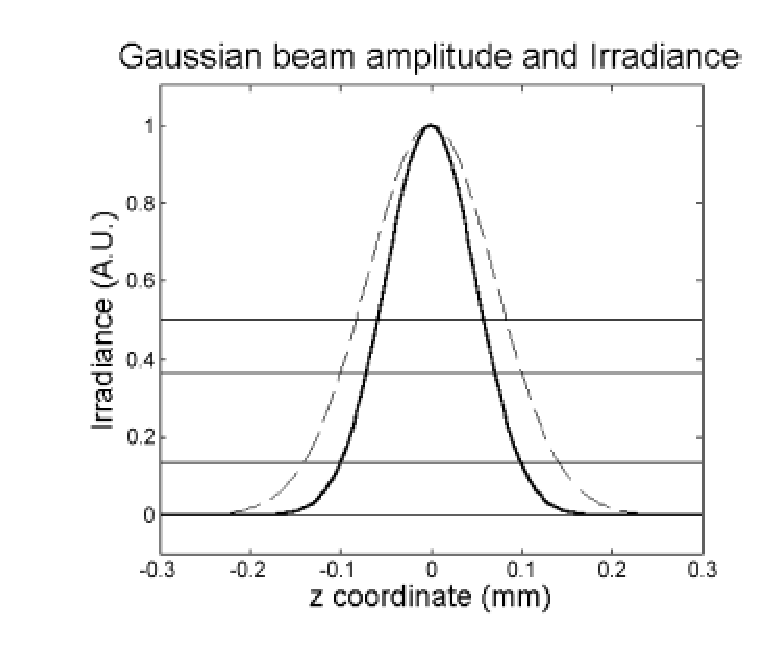
\includegraphics[width=0.8\textwidth]{bilder/gussian_verteilung}
\caption{Transversal profie of the Gussian beam amplitude at the beam waist (dashed line) and irradiance (solid line). Both of them have been normalized to the maximum value. The value of the width of the beam waist $\omega_{0}$ is 0.1 mm. The horizontal lines represent  (in increasing value)the $1/e^{2}$ of the maximum irradiance, the $1/e$ of the maximum amplitude, and the 0.5 of the maximum irrance and amplitude.}
\label{discretization_material}
\end{figure}

%\newpage
%\section{Finite Integration Method}
%%FIT

%\begin{align}
%%\[
%\oint_{\partial A}\vec{E}\cdot\mathrm{d}\vec{s}=
%-\frac{\mathrm{d}}{\mathrm{d}t}\int_{A}\vec{B}\cdot\mathrm{d}\vec{A}\\
%%\]
%%\\
%%\[
%\oint_{\partial A}\vec{H}\cdot\mathrm{d}\vec{s}=
%\int_{A}(\frac{\partial\vec{D}}{\partial t}+\vec{J})\cdot\mathrm{d}\vec{A}\\
%%\]
%%\\
%%\[
%\oint_{\partial V}\vec{D}\cdot\mathrm{d}\vec{A}=
%\int_{V}\rho\mathrm{d}V\\
%%\]
%%\\
%%\[
%\oint_{\partial V}\vec{B}\cdot\mathrm{d}\vec{A}=0
%%\]
%\end{align}
The Finite Integration Theory(FIT) is a numerical simulation method,which was introduced at 1976 by Thomas Weiland to solving the electromagnetical problems after the Maxwell's functions.

\begin{align}
\oint_{\partial A}\vec{E}\cdot\mathrm{d}\vec{s}&=
-\frac{\mathrm{d}}{\mathrm{d}t}\int_{A}\vec{B}\cdot\mathrm{d}\vec{A}\\
\oint_{\partial A}\vec{H}\cdot\mathrm{d}\vec{s}&=
\int_{A}(\frac{\partial\vec{D}}{\partial t}+\vec{J})\cdot\mathrm{d}\vec{A}\\
\oint_{\partial V}\vec{D}\cdot\mathrm{d}\vec{A}&=
\int_{V}\rho\mathrm{d}V\\
\oint_{\partial V}\vec{B}\cdot\mathrm{d}\vec{A}&=0
\end{align}



%fig: discretization of the material
\begin{figure}
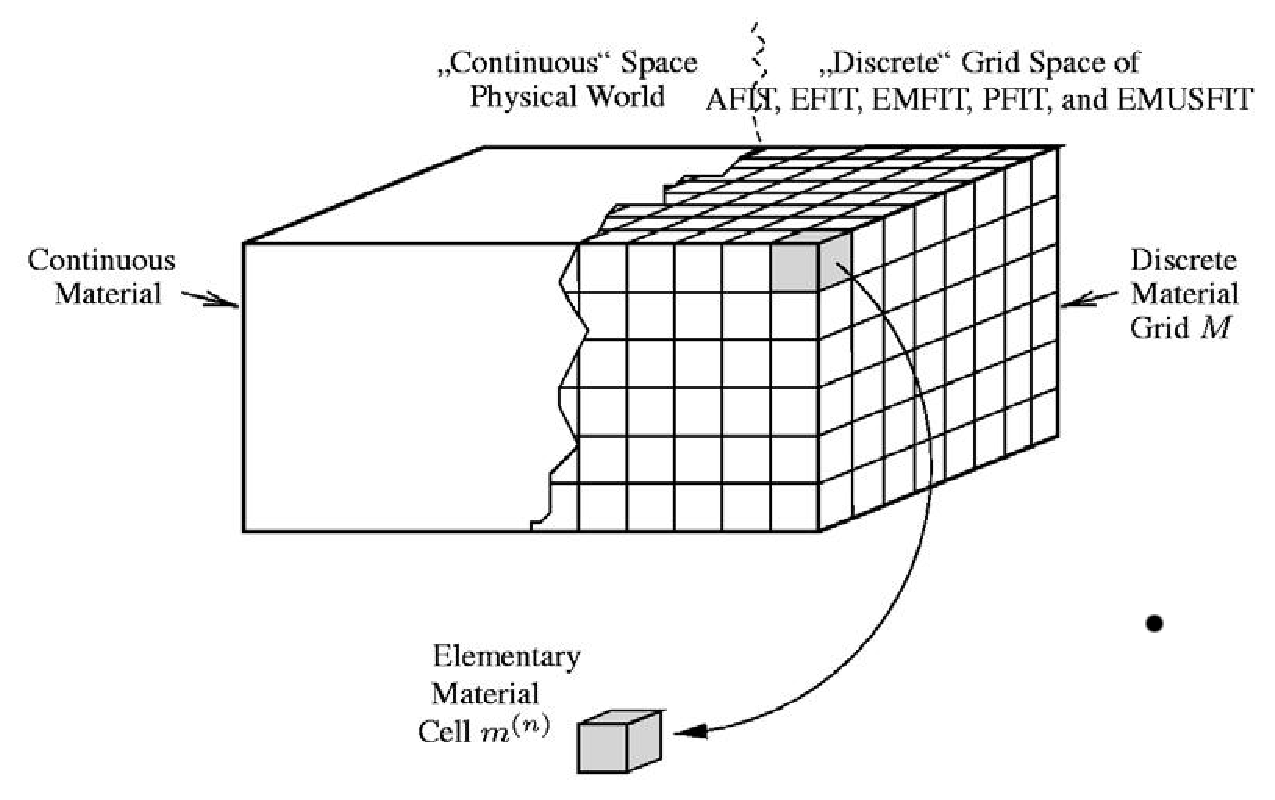
\includegraphics[width=0.8\textwidth]{bilder/discretization_material}
\caption{A discretization of the material in elementary material cells m, defining the material grid M.}
\label{fig:discretization_material}
\end{figure}



%%%law inductive

Following is a demonstration of the discretized form from the inductive law (\ref{eq:maxwell_1}). Considering the path integral in a single element edge like Fig.  \ref{fig:FIT_max_integral1}, the left side of (\ref{eq:maxwell_1}) can be presented as  (\ref{eq:inductive_left}). 

\begin{figure}[!ht]
\centering
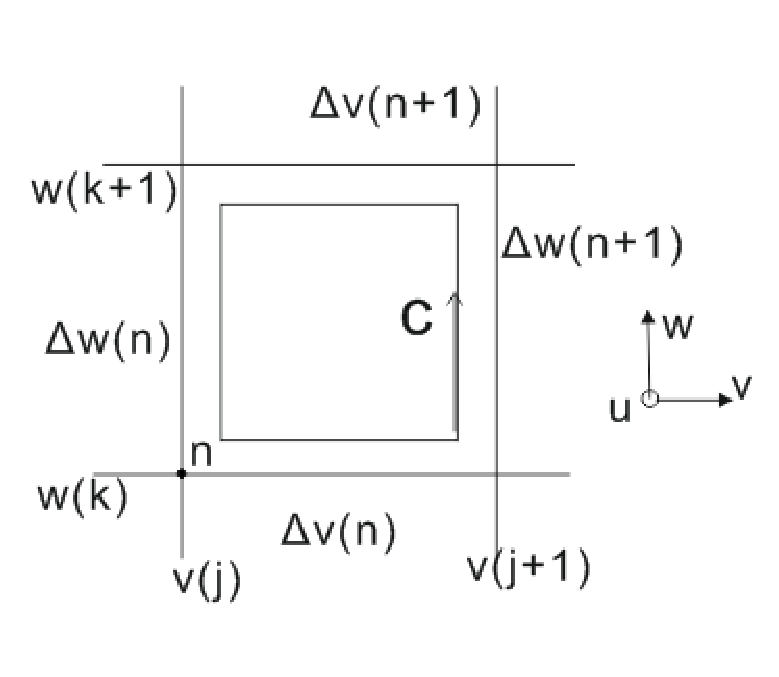
\includegraphics[width=0.45\textwidth]{bilder/FIT_max_integral1}
\caption{ Path integral along edges of one single elemental plane $A_{u}(n)$\cite{ script_FeldSim}.}
\label{fig:FIT_max_integral1}
\end{figure}

\begin{figure}[!ht]
\centering
\subfigure[Discrete electric field strength components distribute at edges of grids.]{
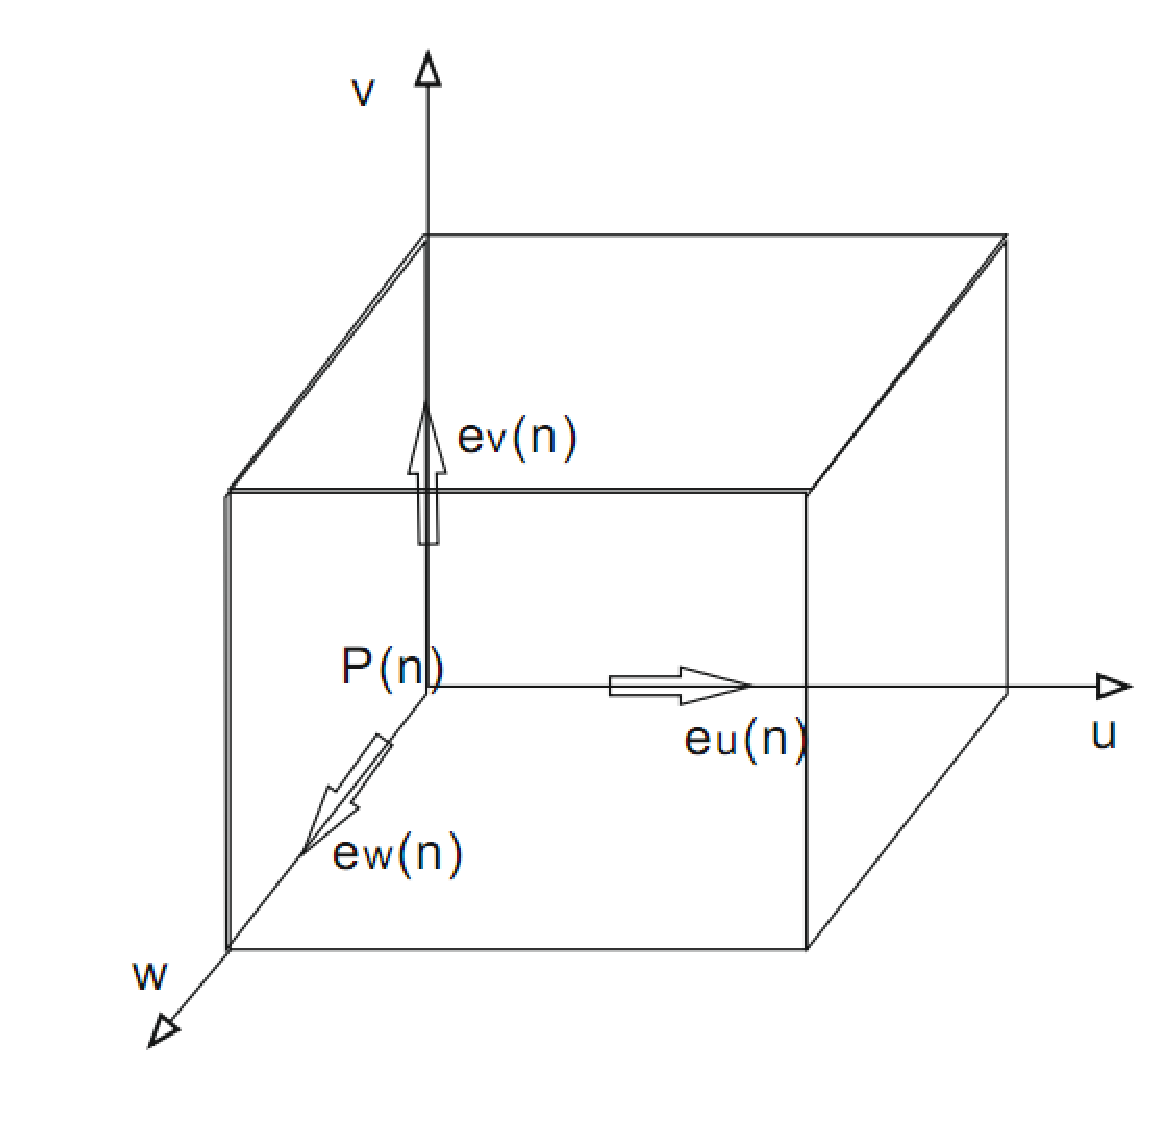
\includegraphics[width=0.4\textwidth]{bilder/FIT_max_integral2}
\label{fig:FIT_max_integral2}
}
\hfill
\subfigure[Discrete magnetic flux density components distribute at planes of grids.]{
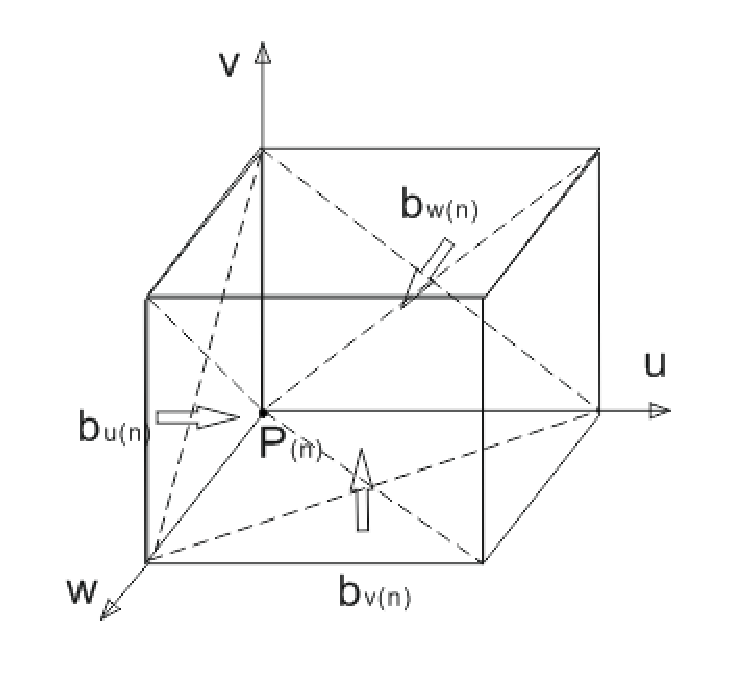
\includegraphics[width=0.5\textwidth]{bilder/FIT_max_integral3}
\label{fig:FIT_max_integral3}
}
\caption{Allocations of components at grids\cite{ script_FeldSim}.}
\end{figure}

\begin{equation}
\int_{C}\vec{E}\cdot d\vec{s}
=\underbrace{\int_{\Delta v(n)}\vec{E}\cdot d\vec{s}}_{\se_{v}(n)}
+\underbrace{\int_{\Delta w(n+M_{v})}\vec{E}\cdot d\vec{s}}_{\se_{w}(n+M_{v})}
-\underbrace{\int_{\Delta v(n+M_{w})}\vec{E}\cdot d\vec{s}}_{\se_{v}(n+M_{w})}
-\underbrace{\int_{\Delta w(n)}\vec{E}\cdot d\vec{s}}_{\se_{w}(n)}
\label{eq:inductive_left}
\end{equation}

Where $\widehat{e}(n)$ is so called  electric grid voltage and has the following relation with electric field strength $e(n)$ (seeing Fig. \ref{fig:FIT_max_integral2})
\begin{equation}
 e_{v}(n)=\frac{\se_{v}(n)}{\Delta v(n)}
\label{eq:e_field}
\end{equation}
Meanwhile the right hand side of (\ref{eq:maxwell_1}) approximates to (\ref{eq:inductive_right})
\begin{equation}
-\iint_{A_{u}(n)}\frac{\partial\vec{B}}{\partial t}\cdot\mathrm{d}\vec{A} 
=-\iint_{A_{u}(n)}\frac{\partial B^{*}_{u}}{\partial t}\cdot\mathrm{d}A
\approx -\frac{\partial}{\partial t}b_{u}(n)A_{u}(n)
\label{eq:inductive_right}
\end{equation}
Where $A_{u}(n)=\Delta v(n)\Delta w(n)$ and $b_{u}(n)$ (Fig. \ref{fig:FIT_max_integral3}) is magnetic flux density, given by
\begin{equation}
 b_{u}(n)=\frac{\widehat{\widehat{b}}_{u}(n)}{\Delta A_{u}(n)} \text{,}
\label{eq:b_flux_density}
\end{equation}
 and magnetic grid flux $\widehat{\widehat{b}}_{u}(n)$, given by
\begin{equation}
\widehat{\widehat{b}}_{u}(n)=\iint_{A_{u}(n)}\vec{B}\cdot\mathrm{d}\vec{A} \text{.}
\label{eq:mag_fluxe}
\end{equation}
From equations (\ref{eq:inductive_left}-\ref{eq:mag_fluxe}) we obtain the difference form (\ref{eq:inductive_integral}) of the inductive equation at one single elemental plane:
\begin{equation}
\widehat{e}_{v}(n)+\widehat{e}_{w}(n+M_{v})-\widehat{e}_{v}(n+M_{w})-\widehat{e}_{w}(n)=-\frac{\partial}{\partial t}\widehat{\widehat{b}}_{u}(n)
\label{eq:inductive_integral}
\end{equation}
i.e.,
\begin{align}
\Delta v(n)e_{v}(n)&+\Delta w(n+M_{v})e_{w}(n+M_{v})\nonumber\\
-\Delta v(n+M_{w})e_{v}(n+M_{w})&-\Delta w(n)e_{w}(n)=-A_{u}(n)\frac{\partial}{\partial{t}}b_{u}(n) 
\label{eq:inductive_sample}
\end{align}
By merging electric field-strength $e(n)$ and magnetic flux density $b(n)$ of all grids into vectors we obtain
\begin{equation*}
e_{u}:=
\begin{pmatrix}
e_{u}(1)&\\
\vdots&\\
e_{u}(N_{p})&
\end{pmatrix},
e_{v}:=
\begin{pmatrix}
e_{v}(1)&\\
\vdots&\\
e_{v}(N_{p})&
\end{pmatrix},
e_{w}:=
\begin{pmatrix}
e_{w}(1)&\\
\vdots&\\
e_{w}(N_{p})&
\end{pmatrix},
e:=
\begin{pmatrix}
e_{u}&\\
e_{v}&\\
e_{w}&
\end{pmatrix},
\label{eq:vector_e_field}
\end{equation*}
\begin{equation*}
b_{u}:=
\begin{pmatrix}
b_{u}(1)&\\
\vdots&\\
b_{u}(N_{p})&
\end{pmatrix},
b_{v}:=
\begin{pmatrix}
b_{v}(1)&\\
\vdots&\\
b_{v}(N_{p})&
\end{pmatrix},
b_{w}:=
\begin{pmatrix}
b_{w}(1)&\\
\vdots&\\
b_{w}(N_{p})&
\end{pmatrix},
b:=
\begin{pmatrix}
b_{u}&\\
b_{v}&\\
b_{w}&
\end{pmatrix}.
\label{eq:vector_m_flux_density}
\end{equation*}
Expanding the relation (\ref{eq:inductive_sample}) to all grid cells \cite{FIT_discrete_method,FIT_discrete_electrommagnetism} we arrive at the discrete form of inductive equation:
\begin{equation}
CD_{s}e=-D_{A}\frac{\partial}{\partial{t}}b
\label{eq:inductive_sample_all}
\end{equation}
Where $D_{s}$ is elemental edge matrix, given by
\begin{align*}
D_{s}=
%	\begin{pmatrix}
%	\Delta u(1)&&&&&&&&\\
%	&\ddots &&&&&&&\\
%	&&\Delta u(N_{p})&&&&&&\\
%	&&&\Delta v(1)&&&&&\\
%	&&&&\ddots &&&&\\
%	&&&&&\Delta v(N_{p})&&&\\
%	&&&&&&\Delta w(1)&&\\
%	&&&&&&&\ddots &\\
%	&&&&&&&&\Delta w(N_{p})
%	\end{pmatrix}
Diag\{&\Delta u(1),\cdots,\Delta u(N_{p}),\nonumber\\
			&\Delta v(1),\cdots,\Delta v(N_{p}),\nonumber\\
			&\Delta w(1),\cdots,\Delta w(N_{p})
\} \text{.}
	%\label{eq:Ds_matrix}
\end{align*}
$D_{A}$ is elemental plane matrix, given by
\begin{align*}
D_{A}=
%	\begin{pmatrix}
%	\Delta A_{u}(1)&&&&&&&&\\
%	&\ddots &&&&&&&\\
%	&&\Delta A_{u}(N_{p})&&&&&&\\
%	&&&\Delta A_{v}(1)&&&&&\\
%	&&&&\ddots &&&&\\
%	&&&&&\Delta A_{v}(N_{p})&&&\\
%	&&&&&&\Delta A_{w}(1)&&\\
%	&&&&&&&\ddots &\\
%	&&&&&&&&\Delta A_{w}(N_{p})
%	\end{pmatrix}
Diag\{&\Delta A_{u}(1),\cdots,\Delta A_{u}(N_{p}),\nonumber\\
			&\Delta A_{v}(1),\cdots,\Delta A_{v}(N_{p}),\nonumber\\
			&\Delta A_{w}(1),\cdots,\Delta A_{w}(N_{p})
\} \text{.}
	%\label{eq:Da_matrix}
\end{align*}
$C$ is \textbf{curl} operator, given by
\begin{equation*}
C=
	\begin{pmatrix}
	0&-P_{w}&P_{v}\\
	P_{w}&0&-P_{u}\\
	-P_{v}&P_{u}&0
	\end{pmatrix} \text{.}
%\label{eq:C_matrix}
\end{equation*}
\begin{figure}[!ht]
\centering
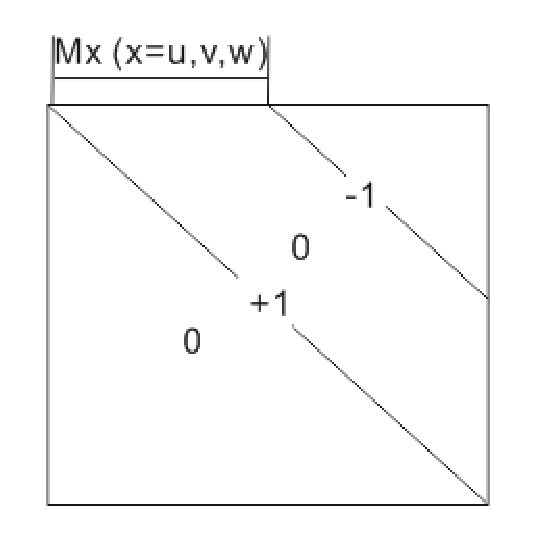
\includegraphics[width=0.35\textwidth]{bilder/P_matrix}
\caption{Structure of matrix $P_{x},(x=u,v,w)$.}
\label{fig:Matrix Px}
\end{figure}
Submatrices $P_{u},P_{v},P_{w}$ are composed of $1,-1,0$ like Fig. \ref{fig:Matrix Px}.\\
 
Alternative form of the equation (\ref{eq:inductive_sample_all}) is given in (\ref{eq:inductive_integral_all})
\begin{equation}
C\widehat{e}=-\frac{\partial}{\partial{t}}\widehat{\widehat{b}}
\label{eq:inductive_integral_all}
\end{equation}
%\widehat{e}
Where $\widehat{e}$ is electric voltage and $\widehat{\widehat{b}}$ magnetic flux.
%divergence equation
Analogy the divergence equation (\ref{eq:maxwell_4}) can also be discretized in grid $G$ and its difference form is given by 
\begin{equation*}
SD_{A}b=0
\label{eq:divergence_sample}
\end{equation*}
or
\begin{equation*}
S\widehat{\widehat{b}}=0
\label{eq:divergence_integral}
\end{equation*}
$S\in \mathbb{R}^{N_{p}\times 3N_{p}}$ represent the discrete divergence matrix, which depends on the grid topology just as the discrete $curl-Matrix$ $C$.
%S
\begin{equation*}
S=(P_{u}|P_{v}|P_{w})
\label{eq:S_matrix}
\end{equation*}
%Amp\'ere's law
For discretizing Amp\'ere's law (\ref{eq:maxwell_2}) \textbf{Dual Grid} is defined, seeing Fig. \ref{fig:dual_grid}. 

\begin{figure}[!ht]
\centering
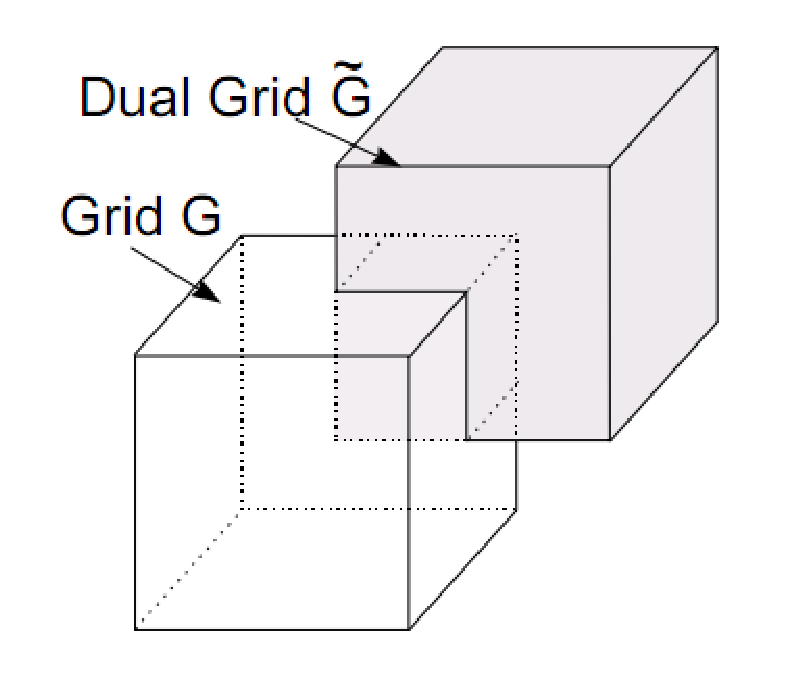
\includegraphics[width=0.5\textwidth]{bilder/dual_grid}
\caption{The allocation of the Primary Grid $G$ and Dual Grid $\tilde{G}$\cite{FIT_discrete_electrommagnetism}.}
\label{fig:dual_grid}
\end{figure}
Then the discretized form of (\ref{eq:maxwell_2}) in dual grid is obtained like
\begin{equation*}
\tilde{C}\tilde{D}_{s}D_{\mu^{-1}}b=\tilde{D}_{A}(D_{\epsilon}\frac{\mathrm{d}}{\mathrm{dt}}e+D_{\kappa}e+j)
\label{eq:ampere}
\end{equation*}
or
\begin{equation*}
\tilde{C}\widehat{h}=\frac{\mathrm{d}}{\mathrm{dt}}\widehat{\widehat{d}}+\widehat{\widehat{j}}_{L}+\widehat{\widehat{j}}_{S}
\label{eq:ampere_sample}
\end{equation*}

Where $\bar{\epsilon}$ is average dielectric constant. $ D_{\epsilon}$ is the average dielectric matrix. $\tilde{C}$ represents the $curl-operator$ in dual grid.
With the help of dual grid cells Gauss' law (\ref{eq:maxwell_3}) in integral form can be discretized\cite{script_FeldSim} as following:
\begin{equation*}
\tilde{S}\widehat{\widehat{d}}=q
\label{eq:gausslaw}
\end{equation*}
or
\begin{equation*}
\tilde{S}\tilde{D}_{A}D_{\epsilon}e=\tilde{D}_{V}\rho_{D}
\label{eq:gausslaw_sample}
\end{equation*}
Where $\rho_{D}$ is the vector of the charge density in grid cells.

\begin{equation*}
\tilde{S}=(\tilde{P}_{u}|\tilde{P}_{v}|\tilde{P}_{w})=(-P_{u}^{T}|-P_{v}^{T}|\-P_{w}^{T})
\label{eq:dual_S_matrix}
\end{equation*}

%%fundamental
%\newpage
%\section{S-Parmeters}
%%S_parameter
Normally an electrical network can be considered as a 'black box', which contains amounts of interconnected basic electrical circuit components such as resistors, capacitors, inductors and transistors etc. On this 'black box' may exist many ports, which present the entries or exits of the network. In order describe the characteristics of this network H-Parameters are used, which describe the relation between voltages and currents. In Fig. \ref{fig:2_port_network} is a 2-port network $V_{1}$ and $V_{2}$ are total voltages of both ports; $I_{1}$ and $I_{2}$ are total currents of both ports respectively. Relations between voltages and currents are like (\ref{eq:voltage_current}). 
\begin{figure}[!ht]
\centering
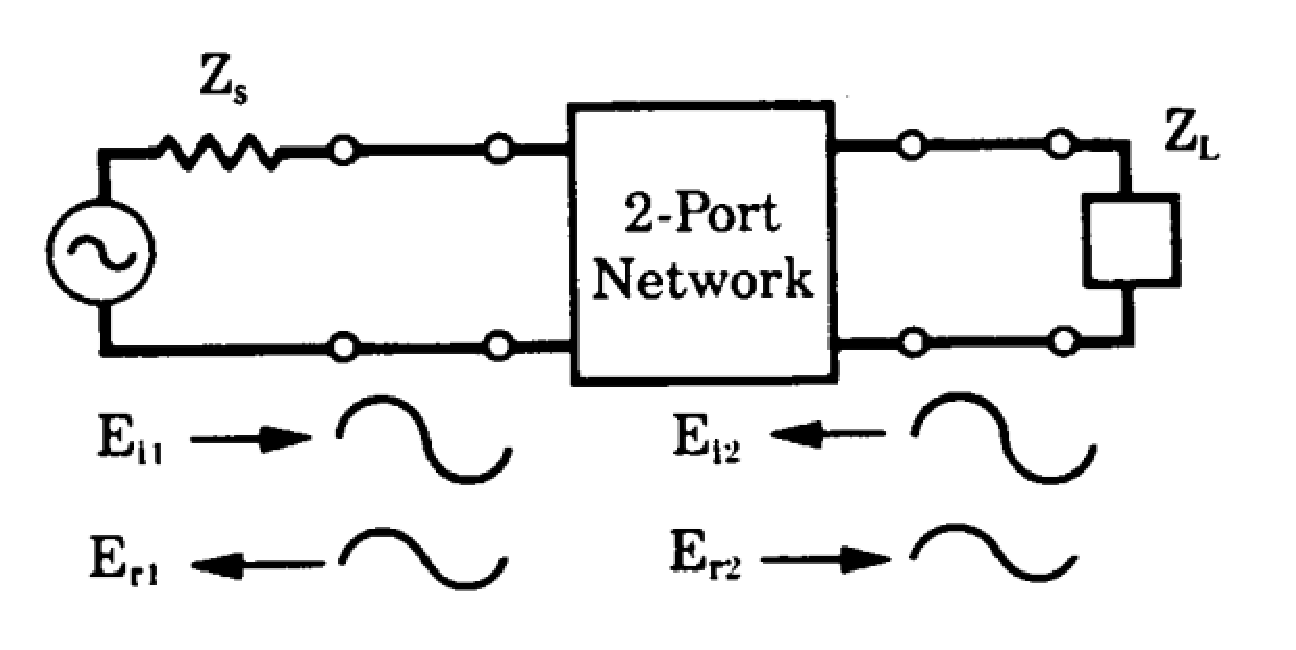
\includegraphics[width=0.6\textwidth]{bilder/s_parameters}
\caption{2-Port-Network \cite{aglient_s_parameters}}
\label{fig:2_port_network}
\end{figure}

\begin{align}
V_{1}&=h_{11}I_{1}+h_{12}V_{2}\\
I_{2}&=h_{21}I_{1}+h_{22}V_{2}
\label{eq:voltage_current}
\end{align}
Where $h_{11},h_{12},h_{21}$ and $h_{22}$ are H-Parameters and defined in (\ref{eq:h_parameters1}-\ref{eq:h_parameters2}).
\begin{align}
h_{11}&=\frac{V_{1}}{I_{1}}|_{V_{2}=0}\quad h_{12}=\frac{V_{1}}{V_{2}}|_{I_{1}=0}
\label{eq:h_parameters1}\\
h_{21}&=\frac{I_{2}}{I_{1}}|_{V_{2}=0}\quad h_{22}=\frac{I_{2}}{V_{2}}|_{I_{1}=0}
\label{eq:h_parameters2}
\end{align}
But H-Parameters cannot always be valid for the description of microwave circuits. Agilent\cite{aglient_s_parameters} has listed some problems of H-Parameters in high frequency:
\begin{itemize}
\item It is not easy to measure the total voltage and total current at the ports of the network.
\item Short and open circuits are not always available for a broad frequency band.
\item For high frequency some circuit are not stable in short or open conditions.
\end{itemize}
Scattering parameters or S-parameters are perfect description of microwave circuit\cite{RF194_s_parameters}. In that case traveling waves are applied instead of total voltages and currents. $E_{i1}$ and $E_{i2}$ represent incidence waves over left and right ports of the network respectively. $E_{r1}$ and $E_{r2}$ are reflective waves. The relation between traveling waves, total voltages and curents has relations (\ref{eq:voltage_wave1}-\ref{eq:voltage_wave2}).
\begin{align}
V_{1}&=E_{i1}+E_{r1}\quad V_{2}=E_{i2}+E_{r2}
\label{eq:voltage_wave1}\\
I_{1}&=\frac{E_{i1}-E_{r1}}{Z_{0}}\quad I_{2}=\frac{E_{i2}-E_{r2}}{Z_{0}}
\label{eq:voltage_wave2}
\end{align}
Traveling waves themselves can be expressed in terms of H-Parameters (\ref{eq:er1}\ref{eq:er2}). 
\begin{align}
E_{r1}&=f_{11}(h)E_{i1}+f_{12}(h)E_{i2}
\label{eq:er1}
\\
E_{r2}&=f_{21}(h)E_{i1}+f_{22}(h)E_{i2}
\label{eq:er2}
\end{align}
Here $f11, f12, f21, f22$ are the network parameters, which indicate the relation between traveling voltages waves and total voltages or currents. Divide both sides of the functions(\ref{eq:er1}-\ref{eq:er2}) by $\sqrt{Z_{0}}$( $Z_{0}$ system impedance).A new set of variables are defined:
\begin{align} 
a1&=\frac{Ei1}{\sqrt{Z_{0}}}=\frac{V_{1}+I_{1}Z_{0}}{2\sqrt{Z_{0}}} \quad a2=\frac{Ei2}{\sqrt{Z_{0}}}=\frac{V_{2}+I_{2}Z_{0}}{2\sqrt{Z_{0}}} \\
b1&=\frac{Er1}{\sqrt{Z_{0}}}=\frac{V_{1}-I_{1}Z_{0}}{2\sqrt{Z_{0}}}  \quad b2=\frac{Er2}{\sqrt{Z_{0}}}=\frac{V_{2}-I_{2}Z_{0}}{2\sqrt{Z_{0}}}
\end{align}
So relations of the new variables are give by:
\begin{align}
b_{1}&=S_{11}a_{1}+S_{12}a_{2}\\
b_{2}&=S_{21}a_{1}+S_{22}a_{2}
\end{align}
or in matrics form:
\begin{equation}
		\begin{pmatrix}
			b_{1}&\\
			b_{2}&
		\end{pmatrix}
	=	
		\begin{pmatrix}
			S_{11}&S_{12}\\
			S_{21}&S_{22}
		\end{pmatrix}
		\begin{pmatrix}
			a_{1}&\\
			a_{2}&
		\end{pmatrix}
\label{eq:s_matrix}
\end{equation}

The S-Parameters are defined as following:
\begin{align}
S_{11}&=\frac{b_{1}}{a_{1}}|_{a_{2}=0}\\
S_{21}&=\frac{b_{2}}{a_{1}}|_{a_{2}=0}\\
S_{22}&=\frac{b_{2}}{a_{2}}|_{a_{1}=0}\\
S_{12}&=\frac{b_{1}}{a_{2}}|_{a_{1}=0}
\end{align}
The phical meaning of the S-Parameters are described as following:
\begin{itemize}
\item $S_{11}$ is the input port reflection coefficient
\item $S_{12}$ is the reverse gain
\item $S_{21}$ is the forward gain
\item $S_{22}$ is the output port reflection coefficient
\end{itemize}
In another hand, $S_{21}$ is often used to estimate the transmission ability of a network. Therefore $S_{21}$ equals the coupling efficiency in this work.


\chapter{Modelling}
%Chapter2
%description

In this chapter the configurations of the experimental objects and corresponding technical detail will be at first introduced. Then it will be described the detail how the simulation models are approximated in CST MWS (CST Studio suite 2010) and the some performances of the simulations will also be illustrated in compare with the practical objects, such as working distance, minimum spot size, power distribution, etc .

\newpage
\section{Project description}
%% Problem description
The left side is a lensed tapered fiber as laser source and at the right side at the working distance there is a chip formed waveguide as signal receiver.  The purpose is to find a way to gain optimized coupling efficiency through the simulations in CST MWS Environments. 


Following is a typical demonastration of fiber-to-chip coupling.
\begin{figure}
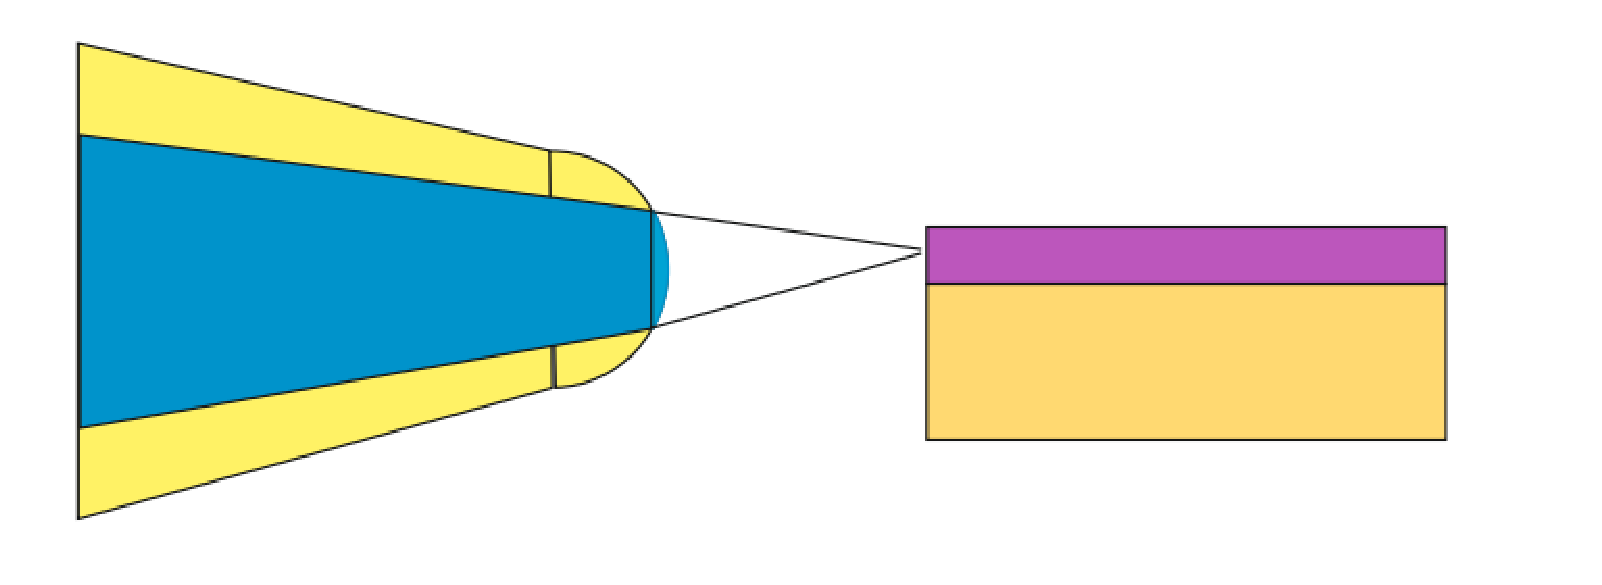
\includegraphics[width=.7\textwidth]{bilder/experiment_object}
\caption{Fiber-to-Chip Coupling}
\label{experiment_object}
\end{figure}

\begin{table}
\begin{tabular}{c|c|c}
\hline
\multicolumn{2}{|c|}{\textbf{Parameter}}&\textbf{Specification(Single-Mode)}\\
\hline
\multirow{3}{*}{Spot Size of Aspheric and Convex Lenses($1/e^2$)}&\multirow{2}{*}{Minum}&$1.7um(\lambda=1.5um)$\\
&																		 &$0.6um(\lambda=0.6um)$\\
&Maxium															 &$6.0um(\lambda=1.5um)$\\
\hline
\multirow{2}{*}{Spot Size Tolerance}&Without near-field optical characterization &$\pm 0.5um$\\
&With near-field optical characterization &$\pm 0.25um$\\
\hline
\multirow{2}{*}{Working Distance} &Minimum &$5um(\lambda=1.5um)$\\
&																	Maximum &$50um(\lambda=1.5um)$\\
\hline
	

Working Distance&
\end {tabular}
\caption{Technical parameters about tapered lensed fiber.\cite{nanoscal_tapered_fiber}}
\label{technical parameters}
\end{table}% arrange the name to 'project_description' 23.02
%Project description
% Problem description
Coupling single-mode fibers to waveguides (Fiber-to-Chip coupling) by microlenses is a very common problem in integrated optics \cite{ integrated_optics}, in wich waveguides locate on a substrate. By means of this technology the simple and reliable optical system with a small size become possible because a lensed fiber has a minized focal length. In this works the application of the lensed fiber-to-chip will be introduced and it coupling efficiency will be discussed.\\
Fig. \ref{fig:experiment_object} is a schematic demonstration of fiber-to-chip coupling. At the one side there is a lensed tapered fiber as laser source and at another side at the working distance of the fiber there is a buried rib waveguide\cite{integrated_optics} as signal receiver. The purpose of this works is to find a way to gain optimized coupling efficiency through the simulations in CST MWS, which is a electromagnetic simulator basically with the implementation of the Finite Integration Technique (FIT)\cite{cst_help_siulation_method}. 


\begin{figure}[!ht]
\centering
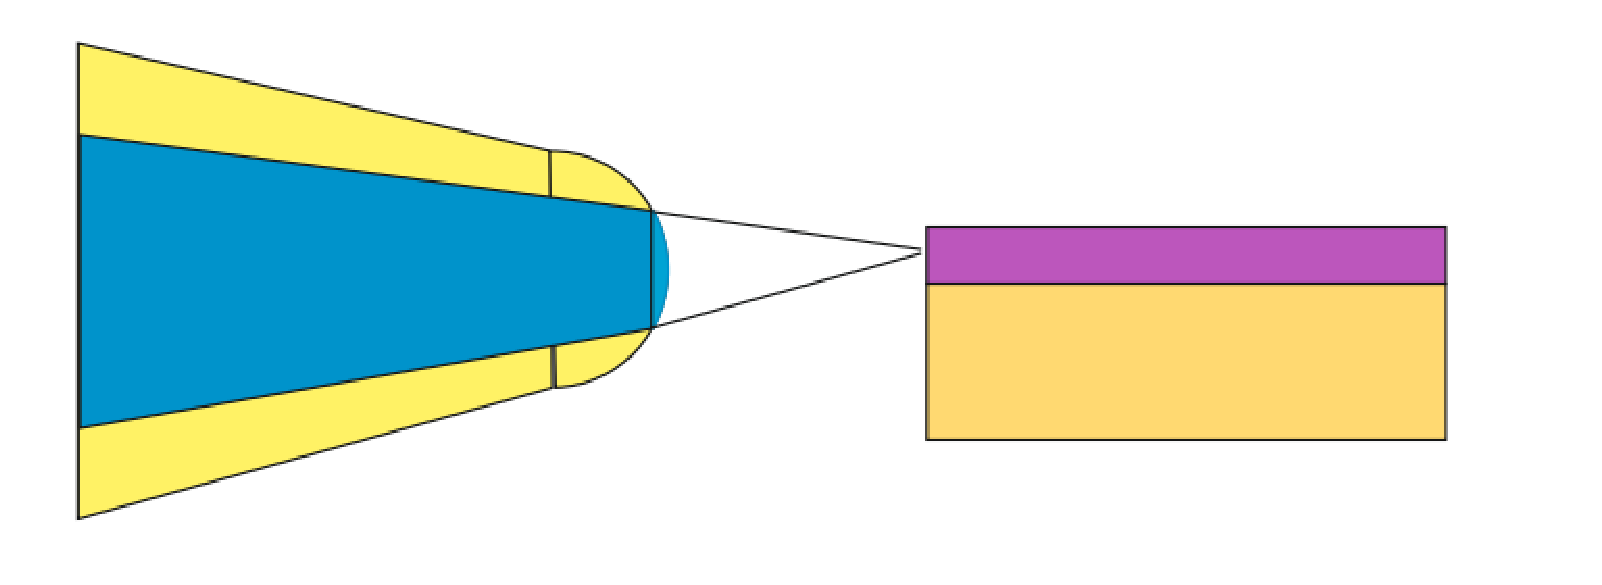
\includegraphics[width=.7\textwidth]{bilder/experiment_object}
\caption{Fiber-to-Chip Coupling}
\label{fig:experiment_object}
\end{figure}

\begin{figure}[!ht]
\centering
\subfigure[Picture of a real Single mode lensed fiber\cite{nanoscal_tapered_fiber}.]{
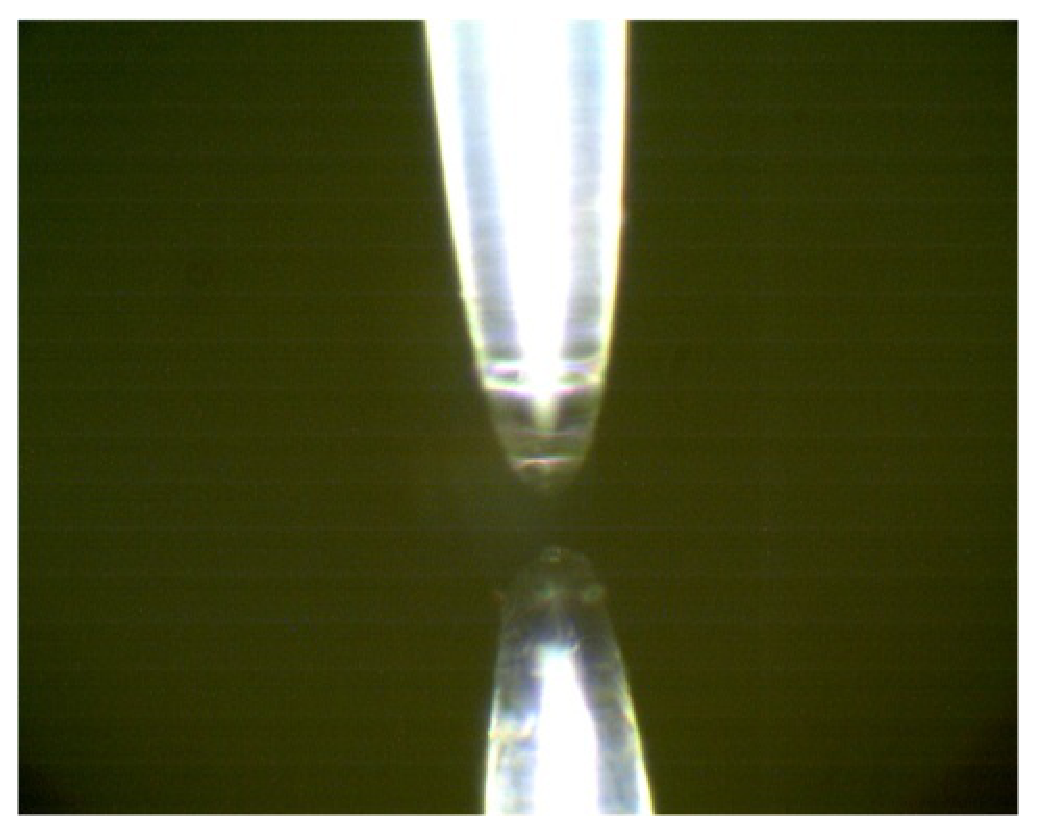
\includegraphics[width=0.3\textwidth]{bilder/single_mode_lensed_fibber}
\label{fig:single_mode_lensed_fiber}
}
\hfill
\subfigure[Schema of a tapered lensed fiber\cite{nanoscal_tapered_fiber}.]{
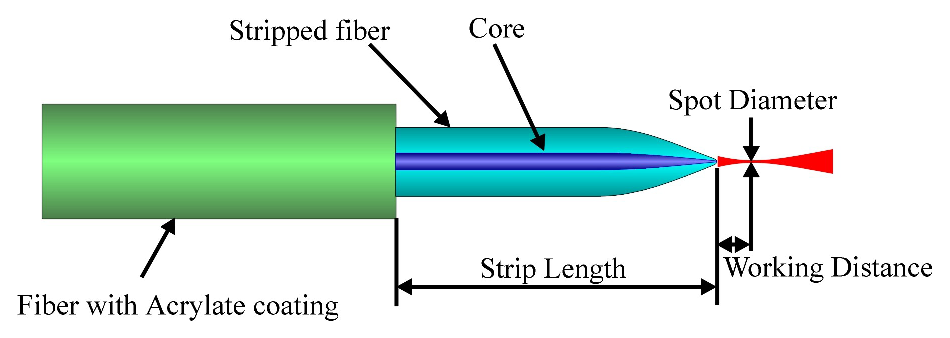
\includegraphics[width=0.6\textwidth]{bilder/tapered_lensed_fiber}
\label{fig:tapered_lensed_fiber}
}
\label{fig:TLFs}
\caption{NANOICS Tapered and Lensed Fibers}
\end{figure}


In this works the the tapered lensed fiber from NANONICS\cite{nanoscal_tapered_fiber} will be used. Fig.\quad\ref{fig:single_mode_lensed_fiber} is the real image of the fiber and Fig.\quad\ref{fig:tapered_lensed_fiber} indicate its schema. In Tab.\quad\ref{tab:technical parameters_lensed_fiber} are listed part of technical parameters, which refer later to the modeling. Additionally the real woking frequence is $\lambda=1064$nm and working distance but $4\mu$m. 
\begin{table}
\caption{Technical parameters about tapered lensed fiber.\cite{nanoscal_tapered_fiber}}
\begin{tabular}{c|c|c}
\hline
\multicolumn{2}{c|}{\textbf{Parameter}}&\textbf{Specification(Single-Mode)}\\
\hline
\multirow{3}{*}{\parbox[t]{0.25\textwidth}{Spot Size of Aspheric and Convex Lenses($1/e^2$)}}&\multirow{2}{*}{Minum}&$1.7\mu$m($\lambda=1.5\mu$m)\\
&																		 &$0.6\mu$m($\lambda=0.6\mu$m)\\
\cline{2-3}
&Maxium															 &$6.0\mu$m($\lambda=1.5\mu$m)\\
\hline
\multirow{2}{*}{Spot Size Tolerance}&\parbox[t]{0.25\textwidth}{Without near-field characterization} &$\pm 0.5\mu$m\\
\cline{2-3}
&\parbox[t]{0.25\textwidth}{With near-field characterization} &$\pm 0.25\mu$m\\
\hline
\multirow{2}{*}{Working Distance} &Minimum &$5\mu$ m($\lambda=1.5\mu$m)\\
\cline{2-3}
&																	Maximum &$50\mu$ m($\lambda=1.5\mu$m)\\
\hline
\end {tabular}

\label{tab:technical parameters_lensed_fiber}
\end{table}

\begin{figure}
\centering
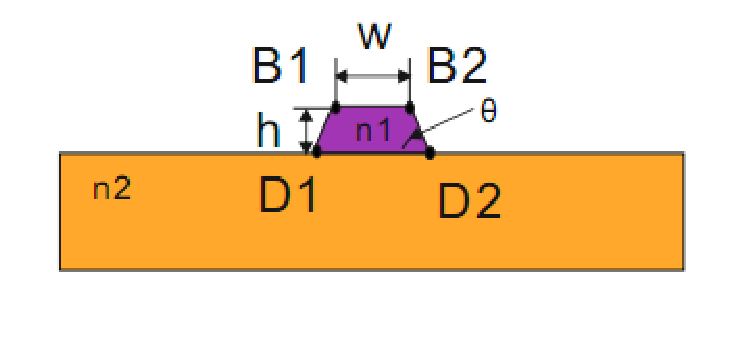
\includegraphics[width=0.4\textwidth]{bilder/orignial_waveguide}
%\subfigure[Schema of a real waveguide.]{
%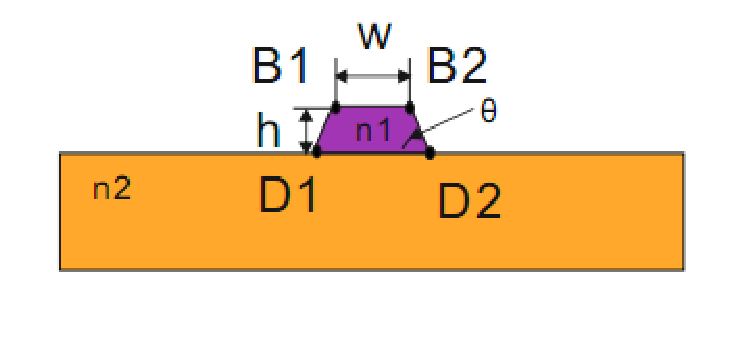
\includegraphics[width=0.4\textwidth]{bilder/orignial_waveguide}
%\label{fig:orignial_waveguide}
%}
%\hfill
%\subfigure[Schema of a approxmate waveguide.]{
%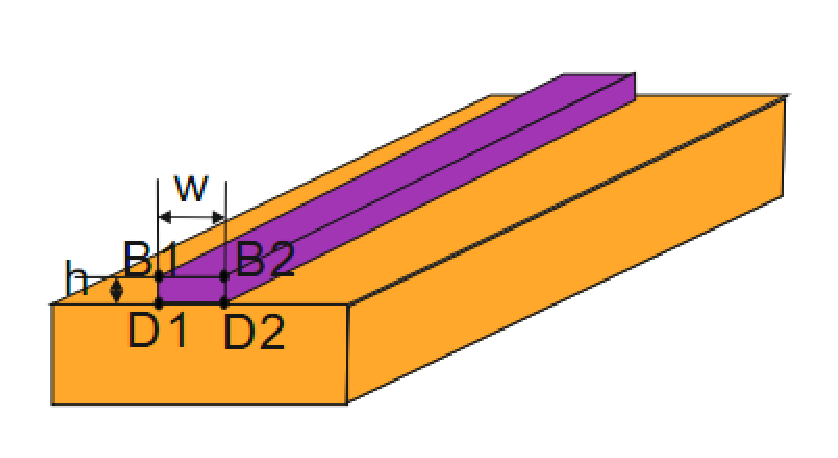
\includegraphics[width=0.4\textwidth]{bilder/approxmate_waveguide}
%\label{fig:approxmate_waveguide}
%}
\caption{Schema of the photonic waveguide}
\label{fig:photonic_waveguide}
\end{figure}
The practical waveguide Fig. \ref{fig:orignial_waveguide} is a trapezoid guide on a semiconductor. But the angles $\theta$ of this guide approximate to $90^{o}$ and is not easy to measure because of its micro-size. Thus a simplified guide model Fig.\ref{fig:approxmate_waveguide} will be used in this works. And the detailed technical properties of the photonic waveguide are given:
\begin{itemize}
\item Working frequency: $\lambda=1064\mu$m
\item Waveguide: LiNbO$_{3}$ with $n_{1}=2.516, w\approx 1\mu$m, $h\approx 0.5 \mu$m
\item Substrate: SiO$_{2}$ with $n_{2}=1.544 $
\end{itemize}

\newpage
\section{Modelling}
%modeling_introduction
For an economic simulation there is no need to create exactly identical models.  Sometimes only parts of the specifics are requested. In this section the modeling process will be discussed. 
\subsection{Modeling the Lensed Fiber}
%fiber_modeling

%\section{Modeling the Lensed Fiber}

Firstly, it is demanded to determine the Tapered and Lensed Fiber(TLF) model. Because of the heave computing cost creating a full size fiber is not economical. Therefore only the end of the fiber, which provides approximately the equal technical properties, will be modeled in this article. In \cite{TLF_analysis} \cite{TLF_mode_transforming} two type of the TLF configuration are mentioned. 


\begin{figure}
\centering
\subfigure[Tapered cladding TLF.]{
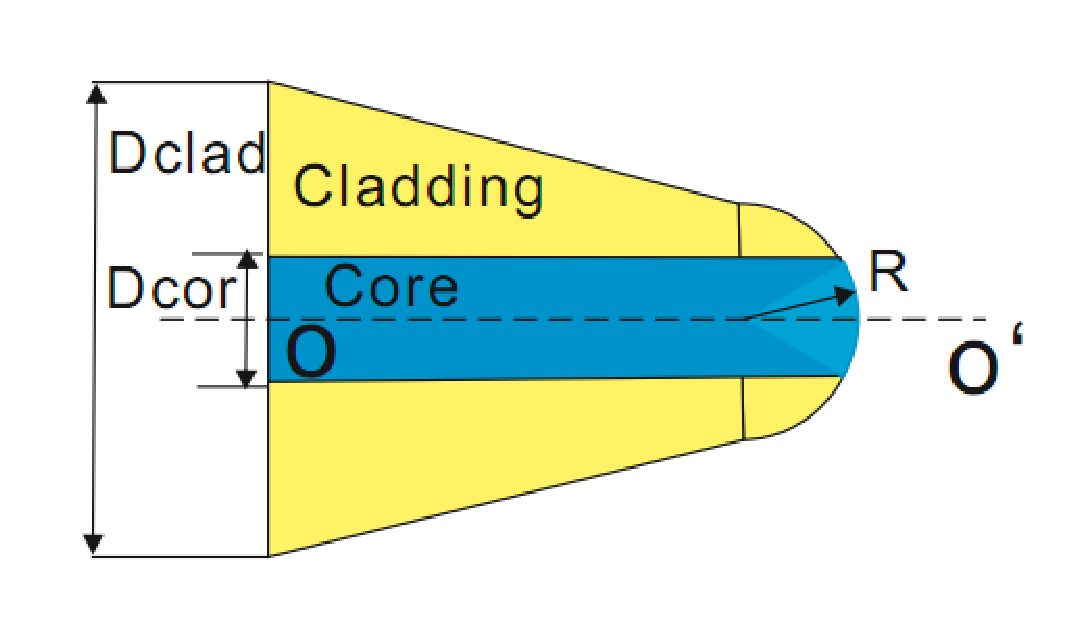
\includegraphics[width=0.4\textwidth]{bilder/lense_fiber_01}
\label{fig:lense_fiber_01}
}
\hfill
\subfigure[Tapered core TLF.]{
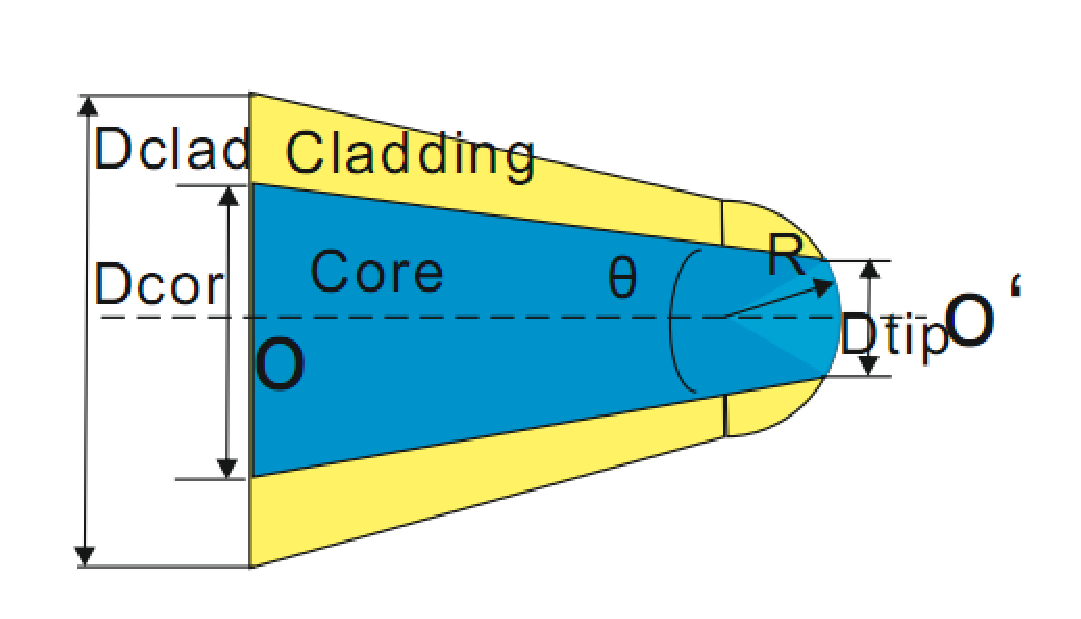
\includegraphics[width=0.4\textwidth]{bilder/lense_fiber_02}
\label{fig:lense_fiber_02}
}
\label{fig:two_TLF}
\caption{Two types of Tapered and Lensed Fibers}
\end{figure}

The Tapered Cladding TLF Fig.\ref{fig:lense_fiber_01} shows that its cladding diameter decreases along the axis and its core diameter is a constant. For the Tapered Core TLF Fig.\ref{fig:lense_fiber_02} its cladding diameter and core diameter both decrease along the axis. \cite{TLF_mode_transforming} develops method to estimate the performance of both type of TLF.  And results show that the performance of the first type of TLF agrees well with the estimation and that of the second type is unpredictable. 

Create two TLF models from each type and test the performances in CST MWS. The following Tab.\ref{tab:model_fiber_configuration} indicates the corresponding configurations.

\begin{table}
\begin{tabular}{ccc}
\hline
							&Tapered Cladding&Tapered Core\\
\hline
$R(\mu m)$ & $6$						 &$6$	\\
refractive indices(core)&$1.68$&$1.66$\\
refractive indices(cladding)&$1.68$&$1.66$\\
$D_{clad}(\mu m)$ &	$17$ &	$17$\\
$D_{core}(\mu m)$ & $10$ &	$17$\\
$D_{tip}(\mu m)$  & --   &	$10$\\
\hline
\end{tabular}
\caption{The Configurations of the TLF Models}
\label{tab:model_fiber_configuration}
\end{table}



\begin{figure}
\setlength{\abovecaptionskip}{0pt}% 
\flushleft
	\subfigure[sub1]{
	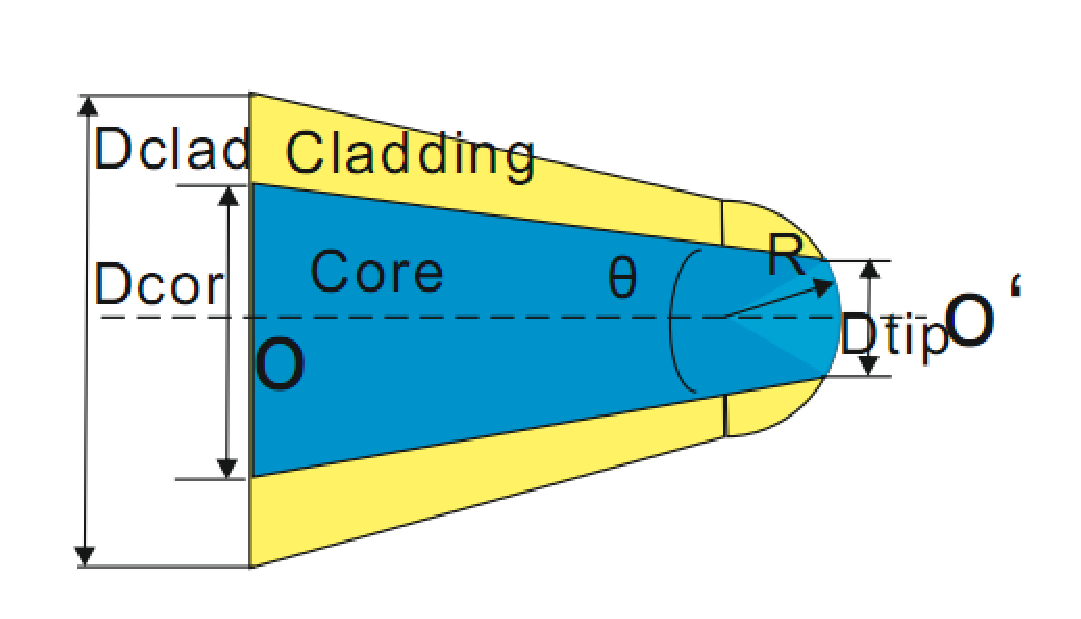
\includegraphics[width=0.23 \textwidth]{bilder/lense_fiber_02}
	\label{fig:subfigure1}%
	}

 	\subfigure[sub2]{
 	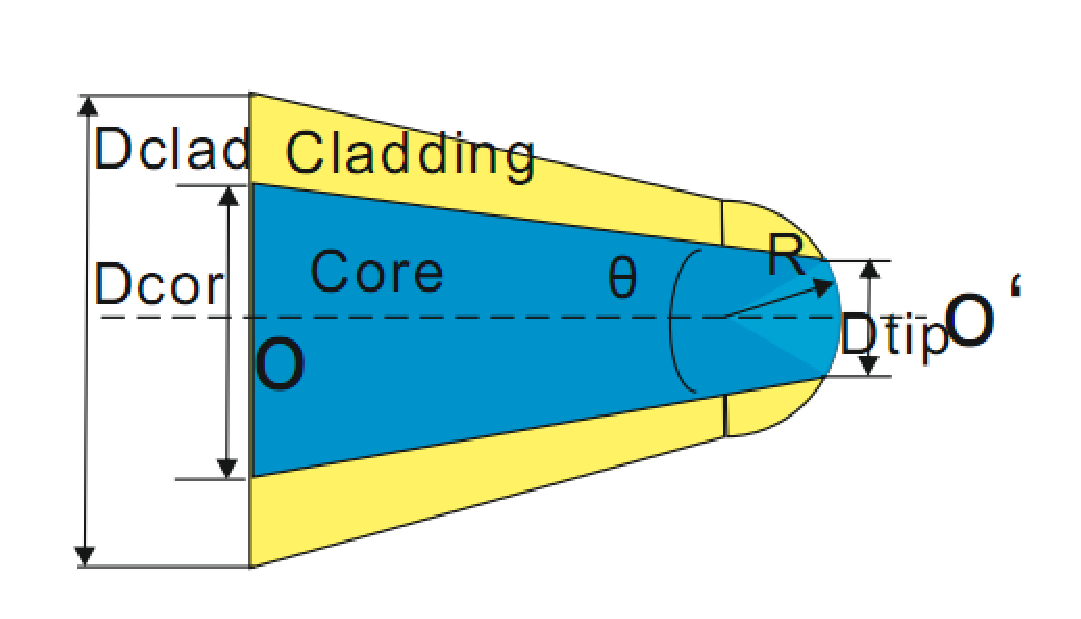
\includegraphics[width=0.23 \textwidth]{bilder/lense_fiber_02}
 	\label{fig:subfigure2}
 	}
 	 	\subfigure[sub2]{
 	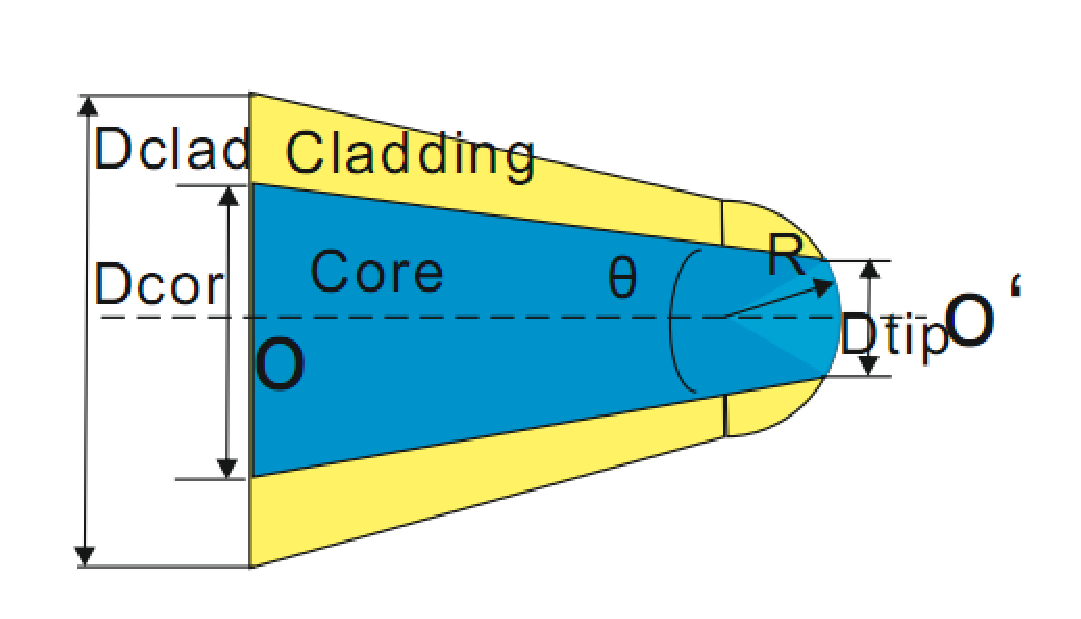
\includegraphics[width=0.23 \textwidth]{bilder/lense_fiber_02}
 	\label{fig:subfigure3}
 	}
 	 	\subfigure[sub2]{
 	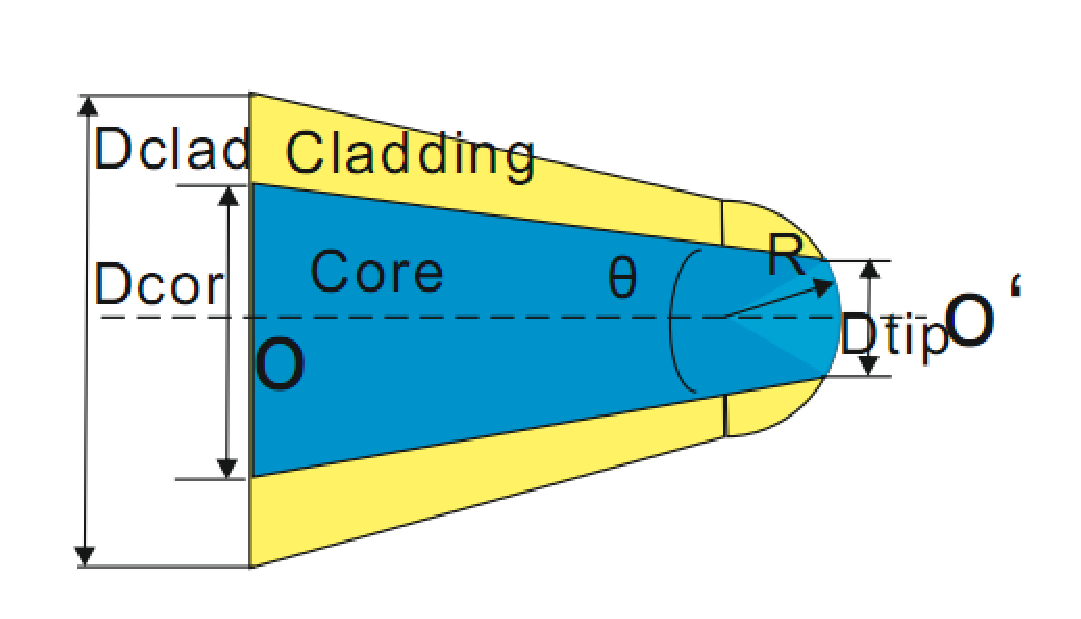
\includegraphics[width=0.23 \textwidth]{bilder/lense_fiber_02}
 	\label{fig:subfigure4}
 	}
 	 	\subfigure[sub2]{
 	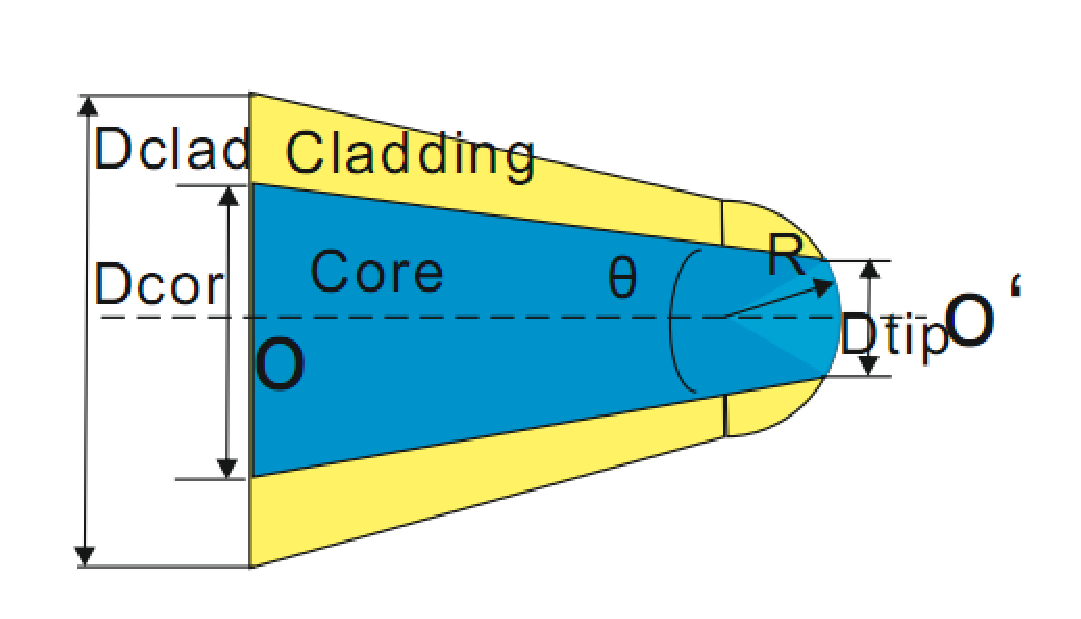
\includegraphics[width=0.23 \textwidth]{bilder/lense_fiber_02}
 	\label{fig:subfigure5}
 	}
\end{figure}

%2.20
The fowllowing is the E-Field demonstration in the xz-plane.
\begin{figure}
	\subfigure[E-Field demonstration of Tapered cladding TLF]{
		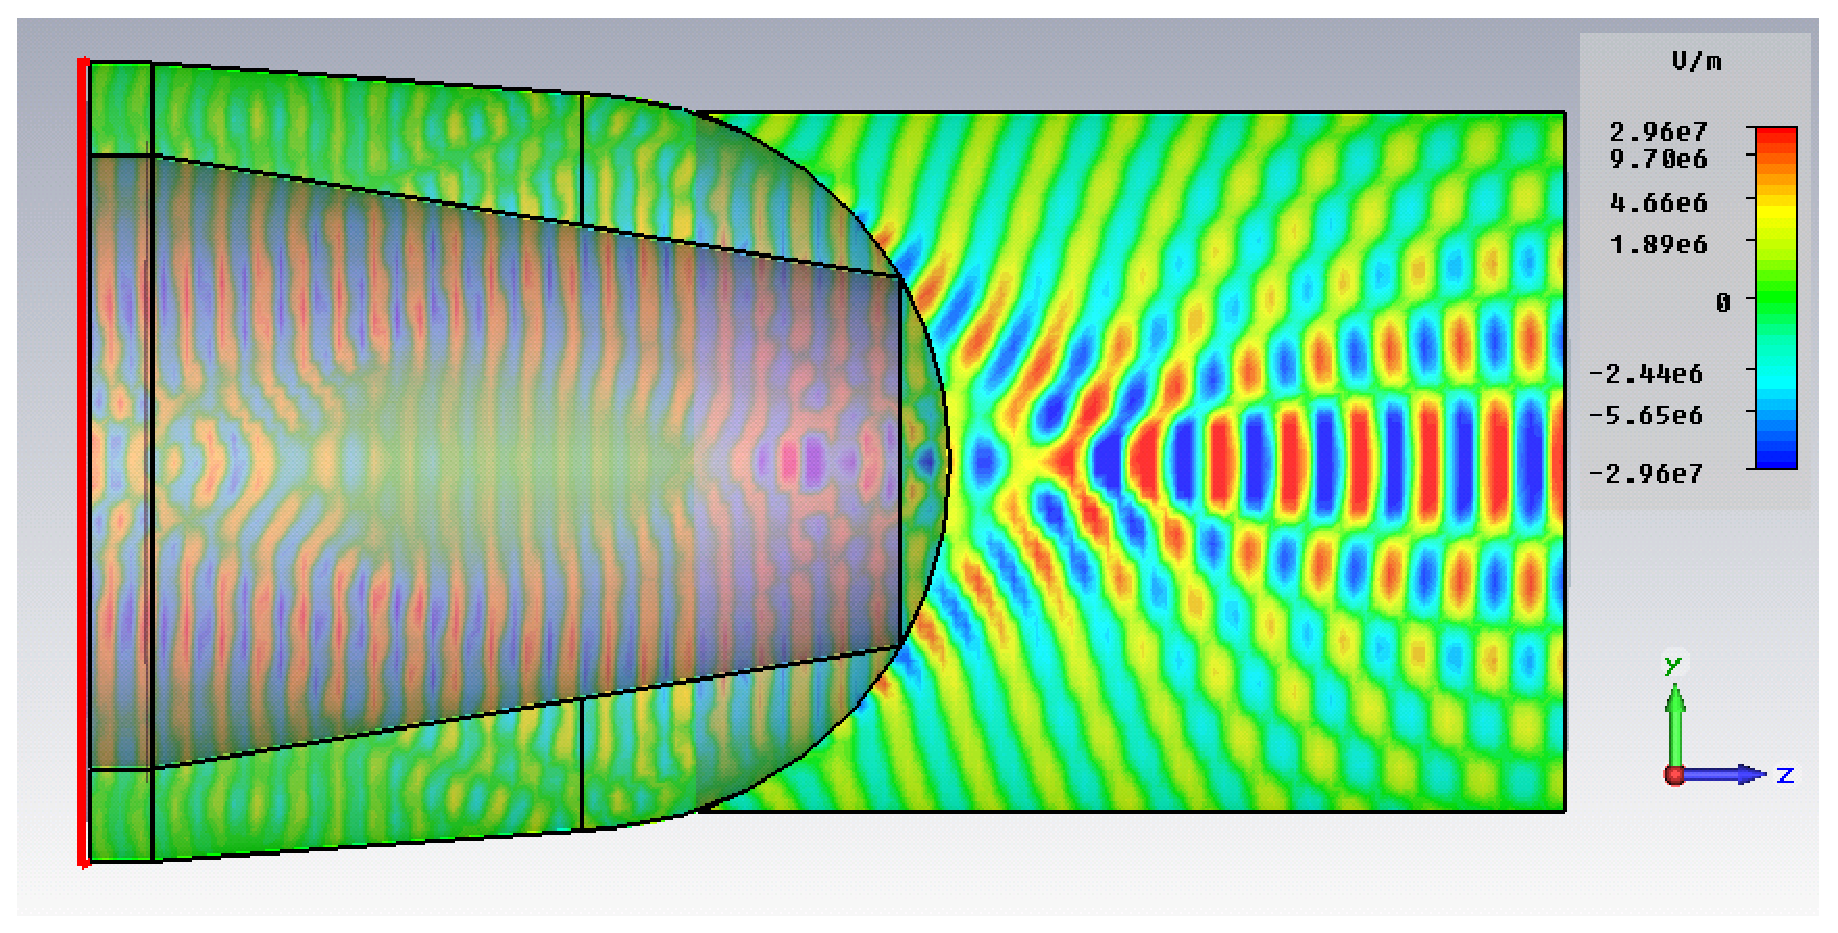
\includegraphics[width=0.4 \textwidth]{bilder/cst_lensed_fiber_efield}
 		\label{fig:Tapered_cladding_efield}
	}
	\subfigure[E-Field demonstration of Tapered core TLF]{
		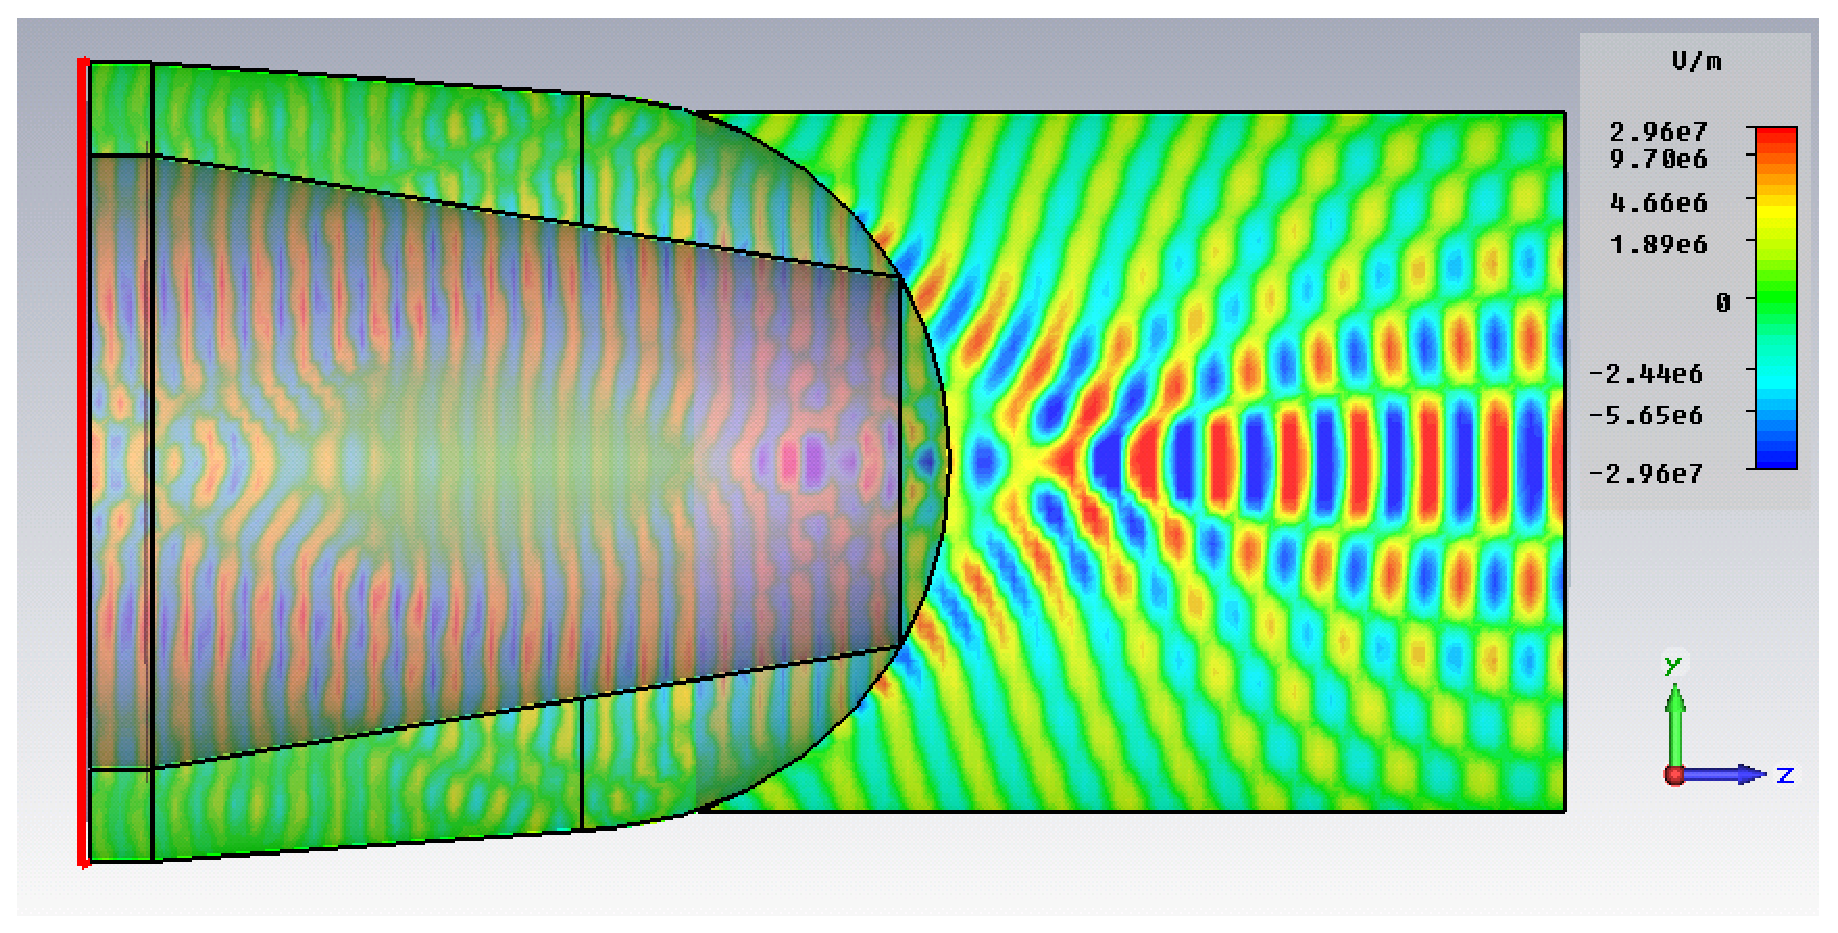
\includegraphics[width=0.4 \textwidth]{bilder/cst_lensed_fiber_efield}
 		\label{fig:Tapered_core_efield}	
	}
	\caption{E Field demonstration}
\end{figure}
As is in section lense theory introduced, the minimum spot located not exactly at the focal length. By using the location of PP and that of MP the MS can be estimated. The theoretical distance from lens end to PP is $xx \mu m$ and the distance from lens end to MP is  $xx \mu m$. Backword $3/4$ LAM form PP, the MS is founded at about $xx \mu m$far from lens end. Through The following figure is the theoretical beam propagation of the lense model.
Load the its beam propagation detail into \textbf{Matlab} workspace and check the beam power distribution in different distance. Fig.(\ref{}-\ref{}).%2D and 3D

\begin{figure}
\end{figure}
 
Draw Fig.\ref{}-\ref{} to illustrate the beam Spot size diameter along the longitude axis.

\begin{figure}
\caption{Curve of Spot size diameter}
\end{figure}
From Fig.\ref{tapered cladding} that the minimum spot size locate at $xxx \mu m$ from lense end and spot size equal about $1.7 \mu m$. While in Fig.\ref{tapered core} that the minimum spot size is found at  $xxx \mu m$ from lense end and spot size equal about $1.5 \mu m$. Thus it is concluded that tapered core TLF has a bit higher focal performance. By rechecking the properties in Tab.\ref{} both TLF model are acceptable for the following development. In this article the Tapered core TLF will be used for further simulations. 

\subsection{Modeling the Fiber to Chip}
%fiber2chip_modelings
As beginning of this chapter the waveguide model will be approximate with a rectangle waveguide. Place the waveguide at the working distance $4\mu$m before the TLF.  Fig.\quad\ref{fig:coupling_e_field} from the simulation of this configuration shows the E-Field spread more widely at the interface of the waveguide than that in the case without blockage of the waveguide and apparently a great part of E-Field infiltrate into the waveguide rather than accepted by guide. Thus by checking the S-parameter of this simulation Fig.\ref{fig:orignial_coupling_efficiency},which present the S21 in frequencies, the coupling efficiency ($S_{21}$) is about $48.8\%$ at the working frequency $282$HZ($\lambda=1064$nm). This result will act as the reference sample for the other simulations. 
\begin{figure}[!ht]
\centering
	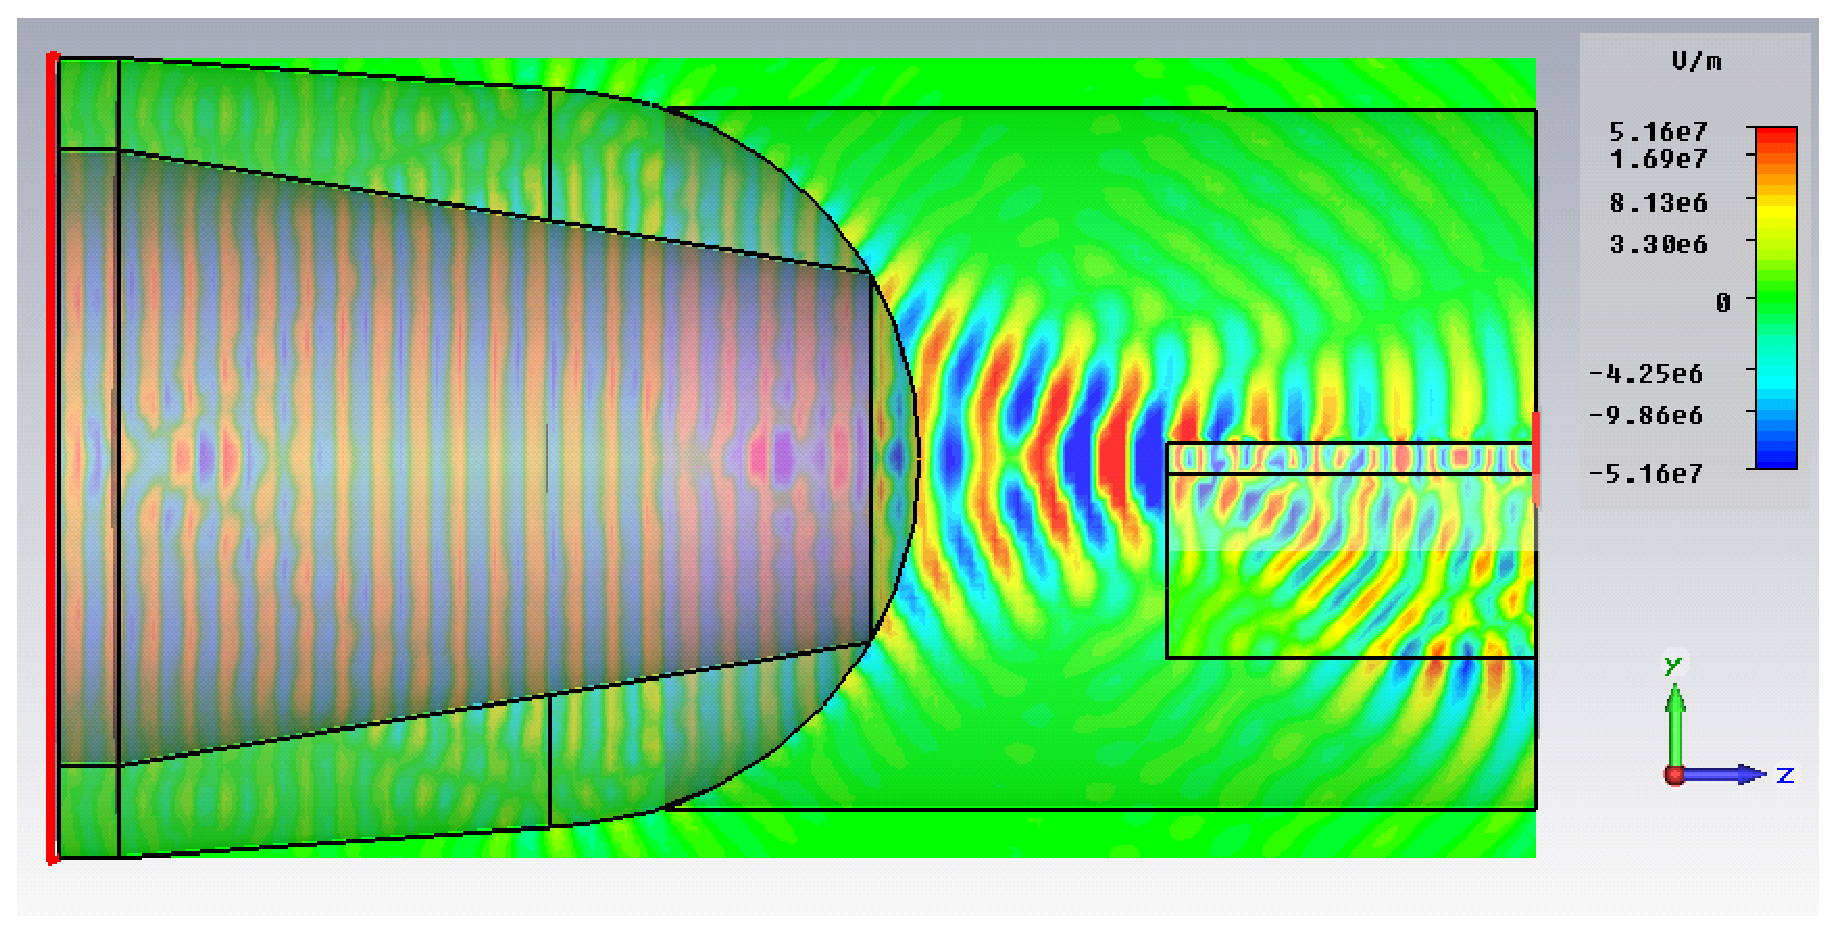
\includegraphics[width=0.7 \textwidth]{bilder/cst_basic_waveguide_efield}
	\label{fig:coupling_e_field}
	\caption{E-Field demonstration by coupling.}
\end{figure}
Furthermore people can analyze the power distribution at the guide from Fig.\quad\ref{fig:power_distribution}( see Appendix.\quad\ref{app:powwer_distribution} ). In the figure it can be found that about $40\%$ power propagates in the guide while another $40\%$ in the substrate and the rest is losing in the air or reflecting.
\begin{figure}
\centering
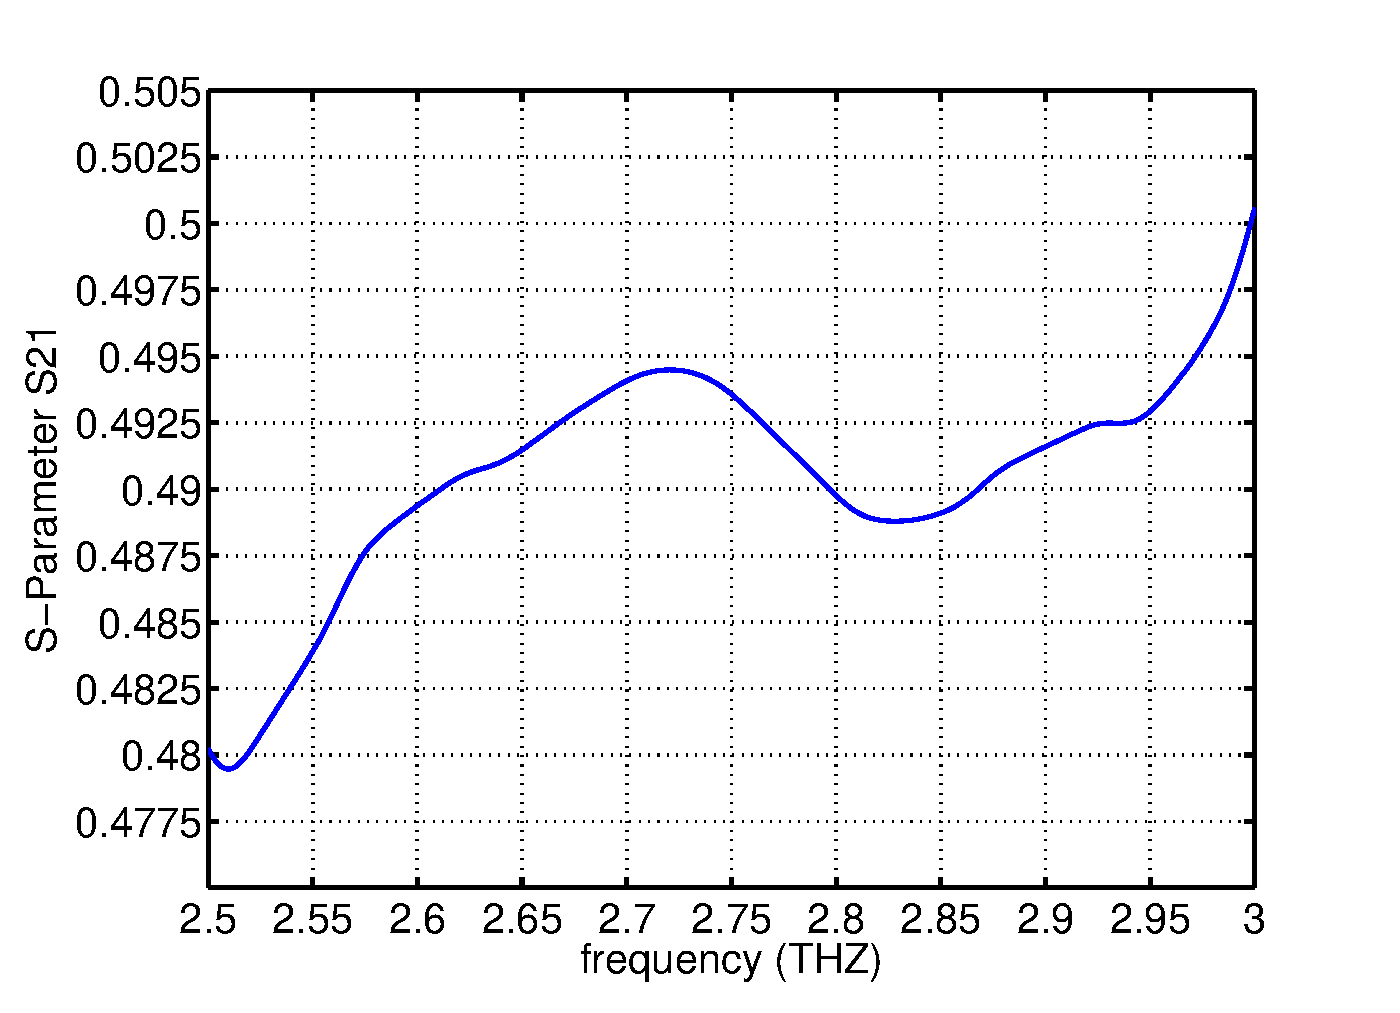
\includegraphics[width=0.7\textwidth]{bilder/original_coupling_efficiency}
\caption{coupling efficiency in Frequency area.}
\label{fig:orignial_coupling_efficiency}
\end{figure}
\begin{figure}[!ht]
\centering
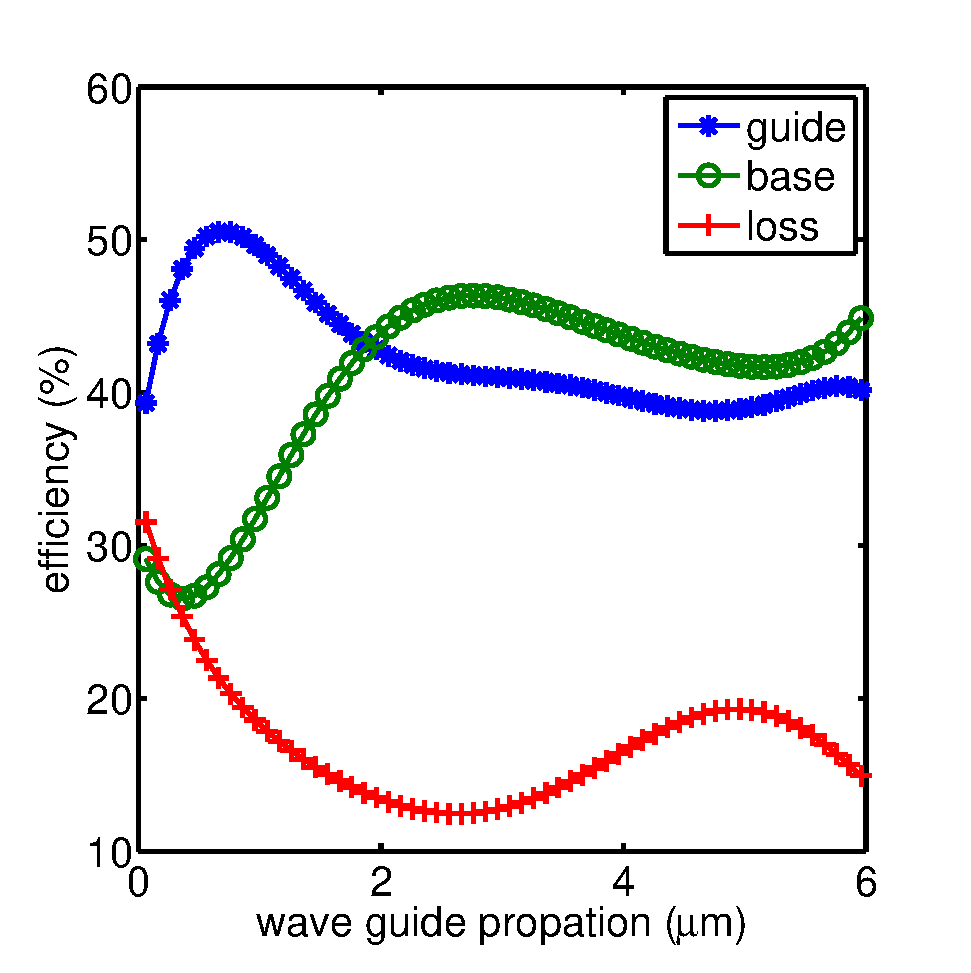
\includegraphics[width=0.7\textwidth]{bilder/power_distribution}
\caption{power distribution along the waveguide.}
\label{fig:power_distribution}
\end{figure}




